%   % !TEX root = ../../VIII,3_Rahmen-TeX_8-1.tex
%
%
%   Band VIII, 3 N.~??S02
%   Signatur/Tex-Datei: LH_35_09_21_001-002
%   RK-Nr. 41201
%   \ref{41201}\ref{RK41201}
%   Überschrift: Leges concursuum
%   Modul: Mechanik / Stoß ()
%   Datierung: ??? Ende Oktober 1686 bis Anfang Februar 1687 ???
%   WZ: (Bl. 1-2) LEd-WZ 803016 = RK-WZ 1192 (insgesamt: eins)
%   SZ:   (?????)
%   Bilddateien (PDF): 
%      LH_35_09_21_001-002_d1 ((ex: lh0350921_001r-d1))
%      LH_35_09_21_001-002_d2 ((ex: lh0350921_002r-d1))
%      (insgesamt: zwei)
%                      
%   Verzeichniseinträge ?????.
%
%
\selectlanguage{ngerman}%
\frenchspacing%
%
%
\begin{ledgroupsized}[r]{120mm}%
\footnotesize%
\pstart%
\noindent\textbf{Überlieferung:}%
\pend%
\end{ledgroupsized}%
\begin{ledgroupsized}[r]{114mm}%
\footnotesize%
\pstart%
\parindent -6mm%
\makebox[6mm][l]{\textit{L}}%
Konzept: LH~XXXV~9,~21 Bl.~1\textendash2.
1 Bogen 4\textsuperscript{o};
ein Wasserzeichen mittig.
Vier Seiten, zweispaltig beschrieben.
Der Text besteht aus mehreren aufeinander folgenden Ansätzen zum selben Gegenstand.
\pend%
\end{ledgroupsized}%
%
%
\vspace*{5mm}%
\begin{ledgroup}%
\footnotesize%
\pstart%
\noindent%
\textbf{Datierungsgründe:}
Das vorliegende Konzept N.~\ref{RK41201} % ??S02 
ist, wie in der Überschrift angegeben, einer Darstellung der Stoßgesetze gewidmet.
Behandelt werden im Text % N.~\ref{RK41201} % ??S02 
lediglich die Gesetze des direkten zentralen Stoßes zweier punktueller Körper.
Hierbei setzt die Darstellung im Wesentlichen die Resultate der auf den Anfang 1678 datierten \textit{Schedae de corporum concursu} \textendash\ insbesondere N.~\ref{dcc_08} % ??S01\textsubscript{10} 
und N.~\ref{dcc_09} %  ??S01\textsubscript{11} 
\textendash\ voraus.
Diese Feststellung stimmt mit der Datierung des Trägers überein, auf dem N.~\ref{RK41201} % ??S02 
überliefert ist:
Dort liegt ein Wasserzeichen vor, das im Nachlass für die zweite Hälfte der 1680er Jahre belegt ist.
Das gleiche Wasserzeichen kommt etwa im Träger des Entwurfs \textit{LSB} VI,~4 N.~303\cite{01355} vor, das editorisch auf \glqq Ende 1685 bis Mitte 1686 (?)\grqq\ datiert wurde.
\pend
\pstart
Weiter einschränken lässt sich die Entstehungszeit von N.~\ref{RK41201} % ??S02 aber 
anhand einer auf Bl.~2~r\textsuperscript{o} vorliegenden Nebenrechnung (siehe die Marginalie zu S.~\refpassage{LH_35_09_21_001-002_c002r9}{LH_35_09_21_001-002_c002r10}).
Diese stimmt nämlich mit einer Rechnung überein, die am unteren Rand von LH~XXXV~9, 20 Bl.~2~v\textsuperscript{o} anzutreffen ist.
Letztere Handschrift überliefert ein Konzept von Leibnizens Rezension zu \protect\index{Namensregister}{\textso{Vanni}, Giovanni Francesco 1638\textendash1709}I.\,F. \textsc{Vanni}, \cite{02000}\textit{Exegeses physico-mathematicae} (Rom 1685), welches samt einer Reinschrift desselben (LH~XXXV~9, 20~Bl.~3\textendash4) und der anonym veröffentlichten Fassung der Rezension (\cite{01023}\textit{AE}, April 1687, S.~197\,f.) voraussichtlich in einem späteren Band von \textit{LSB}~VIII ediert werden soll.
Diese drei überlieferten Entwicklungsstufen der Vanni-Rezension lassen sich fest auf den Zeitraum zwischen Ende Oktober 1686 und Anfang Februar 1687 datieren:
O.~Mencke,%
\protect\index{Namensregister}{\textso{Mencke} (Menken, Menkenius, Menque), Otto 1644\textendash1707}
Hauptherausgeber der \textit{Acta eruditorum}, 
teilte Leibniz in seinem \cite{02013}Brief vom 14.~(24.) Oktober 1686 mit, er habe ihm einige zu besprechende Bücher zugesandt, darunter Vannis \textit{Exegeses}.\cite{02000}%
\protect\index{Namensregister}{\textso{Vanni}, Giovanni Francesco 1638\textendash1709}
Am 2.~(12.) März 1687\cite{02014} bedankte sich Mencke%
\protect\index{Namensregister}{\textso{Mencke} (Menken, Menkenius, Menque), Otto 1644\textendash1707}
dann bei Leibniz für dessen Schreiben vom 11.~(21.) Februar und für die \glqq beygefügten \cite{02023}recensionen\grqq\ (Leibnizens Brief ist nicht erhalten).
Innerhalb dieses Zeitraums müssen alle drei Fassungen der Vanni-Rezension entstanden sein, davon zuerst das Konzept.
\pend
\pstart
Die Rechnung auf LH~XXXV~9, 20 Bl.~2~v\textsuperscript{o} weist keinen Zusammenhang mit dem dort überlieferten Text auf; sie lässt sich indessen als Hilfsrechnung zur genannten Nebenrechnung in N.~\ref{RK41201} % ??S02 
(Marginalie zu S.~\refpassage{LH_35_09_21_001-002_c002r9}{LH_35_09_21_001-002_c002r10}) betrachten.
Aller Wahrscheinlichkeit nach bediente sich Leibniz bei der Abfassung von N.~\ref{RK41201} % ??S02 
des frei gebliebenen unteren Randes der anderen, das Konzept der Vanni-Rezension überliefernden Handschrift, die ihm offenbar zur Hand lag.
Hieraus ergibt sich die für N.~\ref{RK41201} % ??S02 
vorgeschlagene Datierung:
Das Konzept wurde frühestens Ende Oktober 1686 und spätestens Anfang Februar 1687 verfasst.
\pend
\pstart
Erwähnenswert%
\edlabel{LH_35_09_21_001-002_intro_manual-1}
ist schließlich Leibnizens Vermerk am oberen Rand von Bl.~1~r\textsuperscript{o}:
Einen Auszug aus N.~\ref{RK41201} % ??S02 
habe er einem nicht weiter bezeichneten \textit{manuale} hinzugefügt (siehe Randbemerkung zu S.~\refpassage{LH_35_09_21_001r_manuale_obrrnd-1}{LH_35_09_21_001r_manuale_obrrnd-2}).
Damit dürfte wohl dasselbe Hand- und Gedankenbuch gemeint sein, auf das unter dem Begriff \textit{enchiridion} in einem ähnlichen Vermerk zu dem etwas späteren Entwurf N.~\ref{RK60323} (S.~\refpassage{LH_37_05_104r_enchiridion_yfj-1}{LH_37_05_104r_enchiridion_yfj-2}) verwiesen wird.
Worauf sich Leibniz hierbei bezieht, wurde bisher nicht ermittelt.%
\edlabel{LH_35_09_21_001-002_intro_manual-2}
\pend%
\end{ledgroup}%
%
%
\selectlanguage{latin}%
\frenchspacing%
%
%
\count\Bfootins=1100%
\count\Afootins=1200%
\count\Cfootins=1100 
\newpage%
%\vspace*{8mm}
\normalsize%
\pstart%
\noindent%
%
\edtext{}{%
{\xxref{LH_35_09_21_001r_alussa-1}{LH_35_09_21_001r_alussa-2}}%
{\lemma{\lbrack1~r\textsuperscript{o}\rbrack}\Bfootnote{%
\textit{(1)}~Sit cor 
\textit{(2)}~Sint corpora \textit{A}, \textit{B}
\textbar~\textit{(1)}~quorum centrum gravitatis \textit{C}
\textit{(2)}~quorum centrum gra
\textit{erg. u. gestr.}~%
\textbar\ ex primis stationibus \textit{{\scriptsize1}A}, \textit{{\scriptsize1}B}
\textbar~directe \textit{erg.}~%
\textbar\ concurrentia in \textit{{\scriptsize2}A{\scriptsize2}B}
\textbar~seu in \textit{{\scriptsize2}C} \textit{erg.}~%
\textbar\ tempore \textit{{\scriptsize1}C{\scriptsize2}C} velocitatibus \textit{{\scriptsize1}A{\scriptsize2}A} seu \textit{{\scriptsize1}A{\scriptsize2}C}, et \textit{{\scriptsize1}B{\scriptsize2}B} seu \textit{{\scriptsize1}B{\scriptsize2}C}.
\textit{(a)}~Quaeritur
\textit{(b)}~Pon
\textit{(c)}~Magnitudo autem corporum sit talis, ut eorum centrum gravitatis sit \textit{{\scriptsize1}C}, quaer
\lbrack/\rbrack\
\textit{(3)}~Mo\textlangle t\textrangle us definie
\textit{(4)}~Leges concursuum
\lbrack/\rbrack\ Corpora duo \textit{{\scriptsize1}A}
\textbar~et \textit{erg.}~%
\textbar\ \textit{{\scriptsize1}B}, quorum % centrum gravitatis \textit{{\scriptsize1}C}, directe sibi 
\lbrack...\rbrack\ occurrant in
\textit{(a)}~\textit{{\scriptsize1}A{\scriptsize2}B}
\textit{(b)}~\textbar~\textit{{\scriptsize1}A{\scriptsize2}B} \textit{ändert Hrsg.}~%
\textbar\ seu \textit{{\scriptsize2}C},
\textit{(aa)}~celeritatibus \textit{{\scriptsize1}A{\scriptsize2}A},
\textit{(bb)}~nempe \textit{A} celeritate \textit{{\scriptsize1}A{\scriptsize2}A},
\textit{(aaa)}~et \textit{B}
\textit{(bbb)}~seu \textit{{\scriptsize1}A{\scriptsize2}C}, % et \textit{B} celeritate \textit{{\scriptsize1}B{\scriptsize2}B} 
\lbrack...\rbrack\ seu \textit{{\scriptsize1}B{\scriptsize2}C}.
\textit{(aaaa)}~In cent
\textit{(bbbb)}~Sumatur
\textit{(aaaaa)}~${\scriptstyle \textit{2}}C{\scriptstyle \textit{3}}C-{\scriptstyle \textit{2}}C{\scriptstyle \textit{1}}$
\textit{(bbbbb)}~ipsi \textit{{\scriptsize1}C{\scriptsize2}C} aequalis \textit{{\scriptsize2}C{\scriptsize3}C}%
~\textit{L}}}%
}%
%
\lbrack1~r\textsuperscript{o}\rbrack%    %%%%    Blatt 1r
%
\edlabel{LH_35_09_21_001r_alussa-1}%
\edlabel{LH_35_09_21_001r_manuale_obrrnd-1}%
\hspace{45mm}Leges concursuum%
\protect\index{Sachverzeichnis}{lex concursus}%
\protect\index{Sachverzeichnis}{concursus corporum}%
\edlabel{LH_35_09_21_001r_manuale_obrrnd-2}%
%
\edtext{}{%
%{\xxref{LH_35_09_21_001r_manuale_obrrnd-1}{LH_35_09_21_001r_manuale_obrrnd-2}}%
{\lemma{\hspace{1,6mm}\textit{Am oberen Rand:}}\killnumber\Afootnote{%
Hac scheda res omnis recte satis constituta.%
\protect\index{Sachverzeichnis}{scheda excerpta}
Excerptam inde schedam manuali\textsuperscript{[a]} inserui.%
\protect\index{Sachverzeichnis}{manuale}
\newline\vspace{-0.5em}%
\newline%
{\footnotesize%
\textsuperscript{[a]}~manuali:
Nicht ermittelt.
Siehe aber den ähnlichen Hinweis in N.~\ref{RK60323}, S.~\refpassage{LH_37_05_104r_enchiridion_yfj-1}{LH_37_05_104r_enchiridion_yfj-2}.
%??? Dynamica, sezione finale ,De concursu corporum,', LMG 6: 488-514 ???
}%
\newline%
}}}%
%
\pend%
\vspace{0.5em}%
%
%
%  \newpage% 
 % \vspace{0.75em}%
%  \newpage%
%
%
%\begin{center}
%\includegraphics[width=0.7\textwidth]{gesamttex/edit_VIII,3/images/lh0350921_001r-d1.pdf}\\
%\rule[0pt]{0mm}{0pt}[\textit{Fig. 1}]\rule[0pt]{0mm}{0pt}\\
%${\scriptstyle \textit{1}}C{\scriptstyle \textit{2}}C={\scriptstyle \textit{2}}C{\scriptstyle \textit{3}}C$ \textbar\ ${\scriptstyle \textit{1}}A{\scriptstyle \textit{1}}C={\scriptstyle \textit{3}}A{\scriptstyle \textit{3}}C$ \textbar\ ${\scriptstyle \textit{1}}B{\scriptstyle \textit{1}}C={\scriptstyle \textit{3}}B{\scriptstyle \textit{3}}C.$ Ex his  ${\scriptstyle \textit{1}}A{\scriptstyle \textit{1}}B={\scriptstyle \textit{3}}A{\scriptstyle \textit{3}}B.$ ${\scriptstyle \textit{2}}A{\scriptstyle \textit{3}}A\textit{(}v\textit{)},$ ${\scriptstyle \textit{2}}B{\scriptstyle \textit{3}}B\textit{(}y\textit{)}$
%\pend{center}
%
\pstart%
\noindent%
%
% % % %   Achtung getrixt:
\edtext{}{%
\lemma{\hspace{1,6mm}\textit{Unter} \lbrack\textit{Fig.~1}\rbrack:}\killnumber\Afootnote{%
${\scriptstyle\textit{1}}C{\scriptstyle\textit{2}}C = {\scriptstyle\textit{2}}C{\scriptstyle\textit{3}}C$
\textbar\ %%%
${\scriptstyle\textit{1}}A{\scriptstyle\textit{1}}C = {\scriptstyle\textit{3}}A{\scriptstyle\textit{3}}C$
\textbar\ %%%
${\scriptstyle\textit{1}}B{\scriptstyle\textit{1}}C = {\scriptstyle\textit{3}}B{\scriptstyle\textit{3}}C.$%
\textsuperscript{\lbrack a\rbrack}
Ex his
${\scriptstyle\textit{1}}A{\scriptstyle\textit{1}}B = {\scriptstyle\textit{3}}A{\scriptstyle\textit{3}}B.$
\newline\vspace{-0.5em}%
\newline%
{\footnotesize%
\textsuperscript{\lbrack a\rbrack}~%
${\scriptstyle\textit{3}}B{\scriptstyle\textit{3}}C.$~%
\textbar~\textit{(1)}~Unde ${\scriptstyle\textit{1}}A{\scriptstyle \textit{1}}B = \langle{\scriptstyle\textit{3}}A{\scriptstyle\textit{3}}B\rangle$
\textit{(2)}~Unde $\langle{\scriptstyle\textit{1}}A{\scriptstyle\textit{1}}B\rangle$
\textit{(3)}~Ex his ${\scriptstyle\textit{1}}A{\scriptstyle\textit{1}}B = {\scriptstyle\textit{3}}A{\scriptstyle\textit{3}}B.$
\textit{erg.}~\textbar%
~\textit{L}%
}}}%
%${\scriptstyle \textit{2}}A{\scriptstyle \textit{3}}A\textit{(}v\textit{)},$ ${\scriptstyle \textit{2}}B{\scriptstyle \textit{3}}B\textit{(}y\textit{)}$ ???
%
%
Corpora duo \textit{{\scriptsize1}A} et \textit{{\scriptsize1}B},%
\protect\index{Sachverzeichnis}{corpora directe occurrentia}%
\protect\index{Sachverzeichnis}{occursus directus}
quorum centrum gravitatis \textit{{\scriptsize1}C},%
\protect\index{Sachverzeichnis}{centrum gravitatis}
directe sibi occurrant in
\lbrack\textit{{\scriptsize2}A{\scriptsize2}B}\rbrack\
seu \textit{{\scriptsize2}C},
nempe \textit{A} celeritate \textit{{\scriptsize1}A{\scriptsize2}A},
seu \textit{{\scriptsize1}A{\scriptsize2}C},
et \textit{B} celeritate \textit{{\scriptsize1}B{\scriptsize2}B}
seu \textit{{\scriptsize1}B{\scriptsize2}C}.
Sumatur ipsi \textit{{\scriptsize1}C{\scriptsize2}C}
aequalis \textit{{\scriptsize2}C{\scriptsize3}C}%
\edlabel{LH_35_09_21_001r_alussa-2}
%
et ex \textit{{\scriptsize3}C}
sumatur
ad partes \textit{{\scriptsize1}B}
recta ${\scriptstyle\textit{3}}C {\scriptstyle\textit{3}}B
= {\scriptstyle\textit{1}}C{\scriptstyle\textit{1}}B$
rursusque
ad partes \textit{{\scriptsize1}A}
sumatur
ipsa ${\scriptstyle\textit{3}}C {\scriptstyle\textit{3}}A
={\scriptstyle\textit{1}}C{\scriptstyle\textit{1}}A,$
et tempore \textit{{\scriptsize2}C{\scriptsize3}C}
perveniet \textit{A} in \textit{{\scriptsize3}A},
\textit{B} in \textit{{\scriptsize3}B}.
Sive ut enuntiemus generaliter:
si duo
%
\edtext{corpora gravia dura%
\protect\index{Sachverzeichnis}{corpus grave}%
\protect\index{Sachverzeichnis}{corpus durum}%
}{%
\lemma{corpora}\Bfootnote{%
\textit{(1)}~sibi
\textit{(2)}~gravia dura%
~\textit{L}}}
%
in eadem recta
%
\edtext{horizontali}{%
\lemma{horizontali}\Bfootnote{%
\textit{erg.~L}}}
%
concurrant directe,%
\protect\index{Sachverzeichnis}{corpora directe concurrentia}%
\protect\index{Sachverzeichnis}{concursus directus}
centrum gravitatis%
\protect\index{Sachverzeichnis}{centrum gravitatis}
aequaliter progredietur ante et post concursum,%
\protect\index{Sachverzeichnis}{concursus corporum}
et
(\protect\vphantom)%
si corpora ita elastica sint,%
\protect\index{Sachverzeichnis}{corpus elasticum}
ut omnem vim ictus%
\protect\index{Sachverzeichnis}{vis ictus}
percussione sibi impressam%
\protect\index{Sachverzeichnis}{percussio impressa}
in continuationem motus%
\protect\index{Sachverzeichnis}{continuatio motus}
recipiant%
\protect\vphantom()
unumquodque corpus tantum aberit a centro gravitatis%
\protect\index{Sachverzeichnis}{centrum gravitatis}
communi post concursum,
quantum ab eodem aberat aequali tempore ante concursum.%
\protect\index{Sachverzeichnis}{concursus corporum}
\pend%
 \vspace{2.5em}%	% Diagramm 1
  \centerline{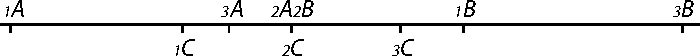
\includegraphics[width=0.8\textwidth]{gesamttex/edit_VIII,3/images/LH_35_09_21_001-002_d1.pdf}}%
  \vspace{0.5em}
  \centerline{\lbrack\textit{Fig.~1}\rbrack}%
  \label{LH_35_09_21_001r_Fig.1}%
\newpage%
%
\count\Bfootins=1000%
\count\Afootins=1200%
\count\Cfootins=1000 
\pstart%
Hoc ita ostendi potest:
Duo corpora \textit{A} et \textit{B}%
\protect\index{Sachverzeichnis}{corpora directe occurrentia}%
\protect\index{Sachverzeichnis}{occursus directus}
sibi occurrere intelligantur in navi \textit{C},%
\protect\index{Sachverzeichnis}{navis}%
\protect\index{Sachverzeichnis}{occursus in navi}
in
%
\edtext{qua eorum centrum gravitatis,%
\protect\index{Sachverzeichnis}{centrum gravitatis}
idque celeritatibus % ,
reciprocis magnitudinum,%
\protect\index{Sachverzeichnis}{celeritas reciproca magnitudini}%
\protect\index{Sachverzeichnis}{magnitudo reciproca celeritati}%
\protect\index{Sachverzeichnis}{celeritas corporum occurrentium}
\textit{A} celeritate \textit{{\scriptsize1}A{\scriptsize1}C},
et \textit{B} celeritate \textit{{\scriptsize1}B{\scriptsize1}C}%
\lbrack;\rbrack% ,
}{%
\lemma{qua}\Bfootnote{%
\textit{(1)}~earum ce
\textit{(2)}~eorum centrum gravitatis,
\textit{(a)}~si ma
\textit{(b)}~idque celeritatibus reciprocis
\textit{(aa)}~, seu quae sint ut \textit{{\scriptsize1}A{\scriptsize1}C}
\textit{(bb)}~magnitudinum, \textit{A} % celeritate \textit{{\scriptsize1}A{\scriptsize1}C} et \textit{B} 
\lbrack...\rbrack\ celeritate \textit{{\scriptsize1}B{\scriptsize1}C}% ,
~\textit{L}}}
%
tempore \textit{{\scriptsize1}C{\scriptsize2}C} % ,
quo%
\protect\index{Sachverzeichnis}{tempus progressionis}
%
\edtext{navis,%
\protect\index{Sachverzeichnis}{navis}%
\protect\index{Sachverzeichnis}{progressio navis}
adeoque}{%
\lemma{navis,}\Bfootnote{%
\textit{(1)}~seu
\textit{(2)}~adeoque%
~\textit{L}}}
%
et centrum gravitatis%
\protect\index{Sachverzeichnis}{centrum gravitatis}%
\protect\index{Sachverzeichnis}{progressio centri gravitatis}%
\lbrack,\rbrack\
progreditur ex \textit{{\scriptsize1}C} in \textit{{\scriptsize2}C},
patet
%
\edtext{motum absolutum%
\protect\index{Sachverzeichnis}{motus absolutus}%
}{%
\lemma{motum}\Bfootnote{%
\textit{(1)}~verum
\textit{(2)}~absolutum%
~\textit{L}}}
%
fore \textit{{\scriptsize1}A{\scriptsize2}A},
\textit{{\scriptsize1}B{\scriptsize2}B};
concurrunt enim in navi%
\protect\index{Sachverzeichnis}{navis}%
\protect\index{Sachverzeichnis}{concursus in navi}
in \textit{C}.
Reflectuntur autem%
\protect\index{Sachverzeichnis}{reflexio corporum concurrentium}
qua venere celeritate,%
\protect\index{Sachverzeichnis}{celeritas reflexionis}
si sibi celeritatibus reciprocis occurrant;%
\protect\index{Sachverzeichnis}{celeritas reciproca}
%
\edtext{ut alibi ostendi.}{%
{\lemma{ut}\Bfootnote{%
\hspace{-0,5mm}alibi ostendi.
\textit{erg.~L}}}%
{\lemma{ut alibi ostendi}\Cfootnote{%
Das Theorem folgt aus den Stoßgesetzen, wie sie Leibniz in den \textit{Schedae de corporum concursu}  (Januar bis Februar 1678) erarbeitet hatte.
Vgl. etwa N.~\ref{dcc_08}, %??S01\textsubscript{10}
S.~\refpassage{LH_37_05_086v_velorecipr-1}{LH_37_05_086v_velorecipr-2}.
%??? Siehe aber Hinweis in den Dechales-Auszügen. ???
}}%
}
%
Itaque dum navis%
\protect\index{Sachverzeichnis}{navis}%
\protect\index{Sachverzeichnis}{progressio navis}
progreditur ex \textit{{\scriptsize2}C} in \textit{{\scriptsize3}C},
distantia eorum a centro gravitatis \textit{{\scriptsize3}C}%
\protect\index{Sachverzeichnis}{centrum gravitatis}%
\protect\index{Sachverzeichnis}{distantia a centro gravitatis}
erit eadem quae ante
seu
${\scriptstyle\textit{3}}A {\scriptstyle\textit{3}}C = {\scriptstyle\textit{1}}A {\scriptstyle\textit{1}}C,$
et
${\scriptstyle\textit{3}}B {\scriptstyle\textit{3}}C = {\scriptstyle\textit{1}}B {\scriptstyle\textit{1}}C.$
\pend%
\vspace{1.0em}%
%
\pstart%
\noindent%
\lbrack\textit{Nachfolgend kleingedruckter Text in L gestrichen:}\rbrack\
\pend%
\vspace{0.5em}%
%
\footnotesize%
\pstart%
{\normalsize%
\lbrack\textit{1.~Ansatz:}\rbrack} % Fassung
%
Calculo rem ita%
\protect\index{Sachverzeichnis}{calculus}%
\protect\index{Sachverzeichnis}{res calculo aestimata}
%
\edtext{aestimabimus:
Corporum magnitudines}{%
\lemma{aestimabimus:}\Bfootnote{%
\textit{(1)}~Celeritas cor
\textit{(2)}~Corporum magnitudines%
~\textit{L}}}
%
sint \textit{a} et \textit{b},%
\protect\index{Sachverzeichnis}{magnitudo corporum concurrentium}
distantiis a centro gravitatis%
\protect\index{Sachverzeichnis}{centrum gravitatis}
expressae,%
\protect\index{Sachverzeichnis}{distantia a centro gravitatis}
itaque
${\scriptstyle\textit{1}}A {\scriptstyle\textit{1}} C = a,$
${\scriptstyle\textit{1}}B {\scriptstyle\textit{1}}C = b,$
distantia corporum $a+b,$%
\protect\index{Sachverzeichnis}{distantia corporum concurrentium}
celeritas ipsius corporis \textit{A} sit \textit{v},
corporis \textit{B}%
\protect\index{Sachverzeichnis}{celeritas corporum concurrentium}
%
\edtext{sit \textit{y},
nempe
$v = {\scriptstyle\textit{1}}A {\scriptstyle\textit{2}}A = {\scriptstyle\textit{1}}A {\scriptstyle\textit{2}}C,$
$y = {\scriptstyle\textit{1}}B {\scriptstyle\textit{2}}B = {\scriptstyle\textit{1}} B{\scriptstyle\textit{1}}C.$
Ponatur autem \textit{v} esse velocitas major,%
\protect\index{Sachverzeichnis}{velocitas major}
fiet
$v \;\pleibdashv\, y = a + b,$%
}{%
\lemma{sit}\Bfootnote{%
\hspace{-0,5mm}\textit{y},
\textit{(1)}~erit $v + y = a + b.$ 
\textit{(a)}~Sit
\textit{(b)}~Si tendunt 
\textit{(aa)}~in easdem partes, vel $\pleibdashv\, v \;\pleibvdash\, y = a + b$
\textit{(bb)}~in contrarias partes
\textit{(2)}~nempe $v = {\scriptstyle\textit{1}}A{\scriptstyle\textit{2}}A = {\scriptstyle\textit{1}}A{\scriptstyle\textit{2}}C,$ $y = {\scriptstyle\textit{1}}B{\scriptstyle\textit{2}}B = {\scriptstyle\textit{1}}B{\scriptstyle\textit{1}}C.$
\textit{(a)}~$v + y =$
\textit{(b)}~Ponatur autem
\textit{(aa)}~corpus
\textit{(bb)}~\textit{v} esse % velocitas major, fiet 
\lbrack...\rbrack\ $v \;\pleibdashv\, y = a + b,$%
~\textit{L}}}
%
et $\pleibdashv$ significat $+$
si corpora sibi occurrunt,%
\protect\index{Sachverzeichnis}{corpora occurrentia}
et $-$
si tendendo in easdem partes%
\protect\index{Sachverzeichnis}{corpora in easdem partes tendentia}
\textit{A} velocitate \textit{v} assequitur \textit{B}.%
\protect\index{Sachverzeichnis}{velocitas assecutionis}
%
\edtext{Centrum gravitatis%
\protect\index{Sachverzeichnis}{centrum gravitatis}
in eam partem tendit
in quam corpus velocius \textit{A}.%
\protect\index{Sachverzeichnis}{corpus velocius}%
}{%
\lemma{Centrum}\Bfootnote{%
\hspace{-0,5mm}gravitatis % in eam partem tendit in quam corpus %
\lbrack...\rbrack\ velocius \textit{A}.
\textit{erg.~L}}}
%
Et celeritas centri gravitatis%
\protect\index{Sachverzeichnis}{celeritas centri gravitatis}
${\scriptstyle\textit{1}} C{\scriptstyle\textit{2}}C = v - a = b \;\pleibvdash\, y$
quam vocemus \textit{c},
%
\edtext{et
${\scriptstyle\textit{1}} C{\scriptstyle\textit{3}}C = 2c,$}{%
\lemma{et}\Bfootnote{\hspace{-0,5mm}%
${\scriptstyle\textit{1}}C {\scriptstyle\textit{3}}C = 2c,$
\textit{erg.~L}}}
%
${\scriptstyle\textit{1}}A {\scriptstyle\textit{3}}C = a + 2c = a + 2v - 2a = 2v - a$
et
${\scriptstyle\textit{3}}C {\scriptstyle\textit{3}}A = a.$
Ergo \textit{{\scriptsize2}C{\scriptsize3}A}
%
\edtext{seu
${\scriptstyle\textit{2}}A{\scriptstyle\textit{3}}A = v - 2a$}{%
\lemma{seu}\Bfootnote{%
\textit{(1)}~${\scriptstyle\textit{2}}A{\scriptstyle\textit{3}}A = v - a$ et ${\scriptstyle\textit{2}}B{\scriptstyle\textit{3}}B = a + b$
\textit{(2)}~${\scriptstyle\textit{2}}A{\scriptstyle\textit{3}}A = v - 2a$%
~\textit{L}}}
%
et
{\normalsize%
\lbrack\textit{Text bricht ab.}\rbrack}%
\pend%
\vspace{1.0em}%
%
\pstart%
{\normalsize%
\lbrack\textit{2.~Ansatz:}\rbrack}
\textit{{\scriptsize1}C{\scriptsize2}C} sit \textit{c},
\textit{{\scriptsize1}A{\scriptsize1}C} sit \textit{a},
\textit{{\scriptsize1}B{\scriptsize1}C} sit \textit{b},
\textit{{\scriptsize1}A{\scriptsize2}A} sit \textit{v},
\textit{{\scriptsize1}B{\scriptsize2}B} sit \textit{y}
{\normalsize%
\lbrack\textit{Text bricht ab.}\rbrack}%
\pend%
\vspace{1.0em}%
%
\pstart%
{\normalsize%
\lbrack\textit{3.~Ansatz:}\rbrack}
Calculo res ita exprimitur%
\protect\index{Sachverzeichnis}{calculus}%
\protect\index{Sachverzeichnis}{res calculo expressa}%
\lbrack:\rbrack\
%\newline%
\textit{{\scriptsize1}C{\scriptsize2}C},
\textit{c} \textbar\ \textit{{\scriptsize1}A{\scriptsize1}C},
\textit{a} \textbar\ \textit{{\scriptsize1}B{\scriptsize1}C},
\textit{b} \textbar\ \textit{{\scriptsize1}A{\scriptsize2}A},
\textit{v} \textbar\ \textit{{\scriptsize1}B{\scriptsize2}B},
$\pleibdashv\; y,$
${\scriptstyle \textit{2}}A{\scriptstyle \textit{3}}A\textit{(}v\textit{)},$
${\scriptstyle \textit{2}}B{\scriptstyle \textit{3}}B\textit{(}y\textit{)}.$
%{\normalsize%
%\lbrack\textit{Text bricht ab.}\rbrack}%
%\pend%
%\vspace{1.0em}%
%
%\pstart%
%{\normalsize%
%\lbrack\textit{4.~Ansatz:}\rbrack}
Cum autem
corporibus duobus in eadem recta concurrentibus%
\protect\index{Sachverzeichnis}{corpora in eadem recta concurrentia}
centrum gravitatis%
\protect\index{Sachverzeichnis}{centrum gravitatis}
semper in eam tendat partem,
in quam tendit corpus % , 
cujus quantitas motus%
\protect\index{Sachverzeichnis}{quantitas motus major}
major est,
id ponatur esse \textit{A},
posito esse $av \,\groesser\, by,$
%
\edtext{et \textit{{\scriptsize1}C{\scriptsize2}C}
sit \textit{c}.
Erit $c=v-a$}{%
\lemma{sit \textit{c}}\Bfootnote{%
\textit{(1)}~$=v-a$
\textit{(2)}~. Erit $c=v-a$%
~\textit{L}}}
{\normalsize%
\lbrack\textit{Text bricht ab.}\rbrack}%
\pend%
\count\Bfootins=1100%
\count\Afootins=1200%
\count\Cfootins=1100 
\newpage%
%
\pstart%
{\normalsize%
\lbrack\textit{4.~Ansatz:}\rbrack}%
\textls{ Centrum gravitatis%
\protect\index{Sachverzeichnis}{centrum gravitatis}
semper in eam tendit partem
in quam tendit corpus,
cujus major est quantitas
%
\edlabel{LH_35_09_21_001r_5Ansatz_mfdf-1}%
motus. }%
\protect\index{Sachverzeichnis}{quantitas motus major}%
%
%
\edtext{}{%
{\xxref{LH_35_09_21_001r_5Ansatz_mfdf-1}{LH_35_09_21_001r_5Ansatz_mfdf-2}}%
{\lemma{\textls{motus}}\Bfootnote{%
\textit{(1)}~\textls{,}~et si quidem corpora ambo in easdem tendant partes tendet eo quo ambo corpora.
\textit{(2)}~\textls{.}~Sin
\textit{(3)}~\textls{.}~Si in contrarias % tendunt partes corpora, centrum gravitatis in contrarias 
\lbrack...\rbrack\ partes movebitur
\textit{(a)}~cum eo cujus
\textit{(b)}~illis in quas % tendit corpus cujus minor est 
\lbrack...\rbrack\ quantitas motus.
\textit{(aa)}~Via centri gravitatis
\textit{(bb)}~Seu si corpora % sibi occurrant, centrum gravitatis praecedit corpus illud 
\lbrack...\rbrack\ cujus major est
\textit{(aaa)}~gravitas
\textit{(bbb)}~motus quantitas, % contrait illi cujus minor. Si corpora tendant 
\lbrack...\rbrack\ in easdem partes,
\textit{(aaaa)}~centrum gravitatis
\textit{(bbbb)}~et major sit quantitas motus corporis praecedentis
\textit{(cccc)}~et tamen % concurrunt, sequens movetur celerius, praecedens tardius. Semper autem centrum gravitatis ibit in easdem partes in quas ambo corpora, eritque 
\lbrack...\rbrack\ via centri gravitatis 
\textit{(aaaaa)}~differentia celeritatum aucta
\textit{(bbbbb)}~aequalis distantiae % corporis praecedentis et 
\lbrack...\rbrack\ viae ejus simul.
\textit{(aaaaa-a)}~Si duo corpora sibi occurrant 
\textit{(bbbbb-b)}~Generaliter,
\textit{(aaaaa-aa)}~si
\textit{(bbbbb-bb)}~corpus
\textit{(ccccc-cc)}~centrum
\textit{(ddddd-dd)}~\textls{via centri gravitatis} est
\textit{(aaaaa-aaa)}~via
\textit{(bbbbb-bbb)}~\textls{excessus celeritatis corporis centrum persequentis supra \textlangle distantiam\textrangle\ a centro}
\textit{(ccccc-ccc)}~differentia inter distantiam corporis
\textit{(aaaaa-aaaa)}~et viam
\textit{(bbbbb-bbbb)}~a centro et % corporis viam; nisi cum centrum gravitatis corpus persequitur, quo casu 
\lbrack...\rbrack\ est eorum summa.%
~\textit{L}}}}%
%
%
Si in contrarias tendunt partes corpora,%
\protect\index{Sachverzeichnis}{corpora in partes contrarias tendentia}
centrum gravitatis%
\protect\index{Sachverzeichnis}{centrum gravitatis}
in contrarias partes movebitur illis
in quas tendit corpus
cujus minor est quantitas motus.%
\protect\index{Sachverzeichnis}{quantitas motus minor}
Seu si corpora sibi occurrant,%
\protect\index{Sachverzeichnis}{corpora occurrentia}%
\protect\index{Sachverzeichnis}{occursus corporum}
centrum gravitatis%
\protect\index{Sachverzeichnis}{centrum gravitatis}
praecedit corpus illud
cujus major est motus quantitas,%
\protect\index{Sachverzeichnis}{quantitas motus major}
contrait illi cujus minor.
Si corpora tendant in easdem partes,%
\protect\index{Sachverzeichnis}{corpora in easdem partes tendentia}
et tamen concurrunt,%
\protect\index{Sachverzeichnis}{corpora concurrentia}
sequens movetur celerius,
praecedens tardius.
Semper autem centrum gravitatis%
\protect\index{Sachverzeichnis}{centrum gravitatis}
ibit in easdem partes in quas ambo corpora,
eritque via centri gravitatis%
\protect\index{Sachverzeichnis}{via centri gravitatis}
aequalis distantiae corporis praecedentis%
\protect\index{Sachverzeichnis}{corpus centrum gravitatis praecedens}%
\protect\index{Sachverzeichnis}{distantia a centro gravitatis}
et viae ejus simul.
Generaliter,% 
\textls{ via centri gravitatis }%
\protect\index{Sachverzeichnis}{via centri gravitatis}%
est differentia inter distantiam corporis a centro et corporis viam;
nisi cum centrum gravitatis%
\protect\index{Sachverzeichnis}{corpus centrum gravitatis persequens}
corpus persequitur,
quo casu est eorum summa.%
\edlabel{LH_35_09_21_001r_5Ansatz_mfdf-2}%
%
\pend%
%
\pstart%
\textls{Si corpora sibi occurrant,%
\protect\index{Sachverzeichnis}{corpora occurrentia}%
\protect\index{Sachverzeichnis}{occursus corporum}
erit summa viarum }%
%
\edtext{%
\textls{aequalis distantiae. }%
\protect\index{Sachverzeichnis}{distantia corporum occurrentium}%
Sin corpus unum}{%
\lemma{\textls{aequalis}}\Bfootnote{%
\textit{(1)}~\textls{summae}
\textit{(2)}~\textls{distantiae}
\textit{(a)}~\textls{a \textlangle cent\textrangle}
\textit{(b)}~Sin corpus unum%
~\textit{L}}}
%
aliud persequatur%
\protect\index{Sachverzeichnis}{corpus aliud persequens}%
\lbrack,\rbrack\
differentia viarum%
\protect\index{Sachverzeichnis}{differentia viarum}
erit aequalis distantiae%
\protect\index{Sachverzeichnis}{distantia a centro gravitatis}
%
\edtext{\lbrack ejus\rbrack}{%
\lemma{ejus}\Bfootnote{%
\textit{erg. Hrsg.}}}
%
quod
%
\edtext{post}{%
\lemma{post}\Bfootnote{\textit{erg.~L}}}
%
centrum gravitatis%
\protect\index{Sachverzeichnis}{centrum gravitatis}
sequitur.
Sit \textit{v} velocitas%
\protect\index{Sachverzeichnis}{velocitas corporum concurrentium}
%
\edtext{corporis \textit{A},
centri via \textit{c},
erit $c = v - a.$
Velocitas autem alterius corporis \textit{B},%
\protect\index{Sachverzeichnis}{velocitas corporum concurrentium}
vocetur \textit{y},
et $a + b = v \;\pleibdashv\, y,$
et $\pleibdashv$ significat $+$
cum corpora sibi occurrunt,%
\protect\index{Sachverzeichnis}{corpora occurrentia}%
\protect\index{Sachverzeichnis}{occursus corporum}
et $-$
cum in easdem partes tendunt.%
\protect\index{Sachverzeichnis}{corpora in easdem partes tendentia}%
}{%
\lemma{corporis}\Bfootnote{%
\textbar\ \textit{A} \textit{erg.}~\textbar~%
\textit{(1)}~cujus
\textit{(a)}~magnit
\textit{(b)}~quantitas motus major
\textit{(2)}~quod semper tendit in eam partem, in quam centrum gravitatis, hujus
\textit{(3)}~centri via \textit{c}.
\textit{(a)}~At alterius corporis via sit $\pleibdashv\, y,$ quae erit $+\,y$ si in easdem partes tendat cum \textit{v} et \textit{c}, et $-\,y$ sin in contrarias, 
\textit{(aa)}~\textlangle\textendash\textrangle\
\textit{(bb)}~$a + b = v \;\pleibdashv\, y$
\textit{(b)}~erit $c = v - a$
\textit{(aa)}~$=\;\pleibdashv\, y - a$
\textit{(bb)}~. Velocitas autem % alterius corporis \textit{B}, 
\lbrack...\rbrack\ vocetur \textit{y},
\textit{(aaa)}~quae sit $+,$ cum in easdem tendit partes, et $-$ cum in contrarias. Jam si corpora
\textit{(aaaa)}~sint
\textit{(bbbb)}~sibi occurrant fit $a + b = v\;\pleibvdash\, y,$ cum tendunt in easdem partes, erit
\textit{(bbb)}~et $a + b = v \;\pleibdashv\, y$ % et $\pleibdashv$ significat $+$ cum corpora sibi occurrunt, et $-$ cum in easdem 
\lbrack...\rbrack\ partes tendunt.%
~\textit{L}}}
%
\pend%
%
\pstart%
Ergo
$c = b \;\pleibvdash\, y,$
%\quad%
%
$\textit{(}v\textit{)} = c - a = v - 2a$
%\quad%
%
seu
$2a = v - \textit{(}v\textit{)},$
%\quad%
%
$\textit{(}y\textit{)} = c + b$
%\quad%
%
seu
$v + \textit{(}y\textit{)} = 2c,$
%\quad%
%
$\textit{(}y\textit{)} = 2b \;\pleibvdash\, y,$
%\quad%
%
seu
$\textit{(}y\textit{)} \;\pleibdashv\, y = 2b$
%\quad%
%
et
$b\textit{(}y\textit{)}\textit{(}y\textit{)} = byy + 4b^3 \;\pleibvdash\, 4b^2y,$
%\quad%
%
$a\textit{(}v\textit{)}\textit{(}v\textit{)} = avv + 4a^3 - 4a^2v$
%\quad%
%
et
$a\textit{(}v\textit{)}\textit{(}v\textit{)} + b\textit{(}y\textit{)}\textit{(}y\textit{)} = av^2 + 4a^3 - 4a^2v + byy + 4b^3 - 4b^2y,$
%\quad%
%
$a^3 - a^2v + b^3 - b^2y$
debet esse $=0,$
%\quad%
%
%\edlabel{LH_35_09_21_001-002_c001v1}%
\textlangle nam\textrangle\
$a^3-a^3-a^2b$
{\normalsize%
\lbrack\textit{Text bricht ab.}\rbrack}
%
{\normalsize%
\lbrack1~v\textsuperscript{o}\rbrack} % % % %    Blatt 1v
%
\pend%
%\vspace{0.75em}%
\newpage
\pstart%
{\normalsize%
\lbrack\textit{5.~Ansatz:}\rbrack}
\quad%
%
%\edtext{}{{\xxref{LH_35_09_21_001-002_c001v1}{LH_35_09_21_001-002_c001v2}}\lemma{nam $a^3-a^3-a^2b$}\Bfootnote{[1~v\textsuperscript{o}]
%\textit{(1)}~
$a+ b = v \;\pleibdashv\, y,$
\quad%
$c = v - a = b \;\pleibvdash\, y,$
\quad%
$\textit{(}v\textit{)}= c - a = v - 2a.$
Unde
$2a = v - \textit{(}v\textit{)}.$
\quad%
$\textit{(}y\textit{)} = c + b = \;\pleibvdash\, y + 2b.$
Unde
$2b = \;\pleibdashv\, y + \textit{(}y\textit{)}$
et
$\textit{(}v\textit{)} - \textit{(}y\textit{)} = v - 2a \;\pleibdashv\, y - 2b = -\,a - b$
seu
%
$\textit{(}y\textit{)} - \textit{(}v\textit{)} =
\edlabel{LH_35_09_21_001v_dfgr-1}%
a + b.$
%
\edtext{}{%
{\xxref{LH_35_09_21_001v_dfgr-1}{LH_35_09_21_001v_dfgr-2}}%
{\lemma{$a + b.$}\Bfootnote{%
\textit{(1)}~(\protect\vphantom)Quod tamen non bene succedit, cum $\textit{(}y\textit{)}+\textit{(}v\textit{)}$ in casu occursus sit $=a+b.$
\textit{(2)}~Et subest quaedam subtilitas\protect\index{Sachverzeichnis}{subtilitas} in
\textit{(a)}~sig
\textit{(b)}~ipsis signis
\textit{(3)}~Est autem % \textit{\textit{(}v\textit{)}} quantitas negativa 
\lbrack...\rbrack\ quando $a\;\groesser\, c.$
\textit{(a)}~$a\textit{(}v\textit{)}\textit{(}v\textit{)}=
\textit{(b)}~\textit{(}v\textit{)}=v-2a$ ut diximus\lbrack,\rbrack\ $\textit{(}y\textit{)}=\;\pleibvdash y + 2b = v - a - b$
\textit{(c)}~Videamus an $avv + byy = a\textit{(}v\textit{)}\textit{(}v\textit{)} + b\textit{(}y\textit{)}\textit{(}y\textit{)}$%
~\textit{L}}}}%
%
Est autem \textit{\textit{(}v\textit{)}} quantitas negativa%
\protect\index{Sachverzeichnis}{quantitas negativa}
quando $a\;\groesser\, c.$%
\pend%
%\newpage%
%
\pstart%
Videamus an
$avv + byy = a\textit{(}v\textit{)}\textit{(}v\textit{)} + b\textit{(}y\textit{)}\textit{(}y\textit{)}$%
\edlabel{LH_35_09_21_001v_dfgr-2}
%
seu an
$a\overline{vv - \textit{(}v\textit{)}\textit{(}v\textit{)}} = b\overline{\textit{(}y\textit{)}\textit{(}y\textit{)} - yy}$
seu
$a : b = \textit{(}y\textit{)}^2 - yy\lrcorner : \llcorner v^2 - \textit{(}v\textit{)}^2.$
Jam
$\textit{(}y\textit{)} - \textit{(}v\textit{)} = \;\pleibdashv\, y + b$
et
$\textit{(}y\textit{)} \;\pleibvdash\, y = v + \textit{(}v\textit{)}.$
Ergo
$a : b = \textit{(}y\textit{)} \;\pleibdashv\, y\lrcorner : \llcorner v - \textit{(}v\textit{)}$
seu
$av - a\textit{(}v\textit{)} = b\textit{(}y\textit{)} \;\pleibdashv\, by$
seu
$av \;\pleibvdash\, by \stackrel{\astrosun}{=}
%
\edtext{a\textit{(}v\textit{)} + b\textit{(}y\textit{)}.$
Unde sequeretur eo casu,%
\protect\index{Sachverzeichnis}{casus}
quo corpora in easdem partes tendunt%
\protect\index{Sachverzeichnis}{corpora in easdem partes tendentia}%
\lbrack,\rbrack\
coincidere summam virium% , %
\protect\index{Sachverzeichnis}{summa virium}
et quantitates motus.%
\protect\index{Sachverzeichnis}{quantitas motus}
Jam
$\pleibdashv\, y = a + b - v$}{%
\lemma{$a\textit{(}v\textit{)} + b\textit{(}y\textit{)}.$}\Bfootnote{%
\textit{(1)}~Jam $\pleibdashv y$
\textit{(2)}~Unde sequeretur
\lbrack...\rbrack\ Jam $\pleibdashv\, y = a + b - v$%
~\textit{L}}}
%
et
$\textit{(}y\textit{)} = v - a + b$
et
$\textit{(}v\textit{)} = v - 2a.$
\pend%
%
\pstart%
Ergo ex aeq. \astrosun\ fiet:
$\protect\ovalbox{$av$} \; \protect\ovalbox{$-\,ab$} \,- bb \; \protect\ovalbox{$+\,bv$} = \protect\ovalbox{$av$} \,- 2aa \; \protect\ovalbox{$+\,bv$} \; \protect\ovalbox{$-\,ba$} \,+ bb$
et fieret
$aa = bb,$
quod est absurdum.%
\protect\index{Sachverzeichnis}{absurdum}
Ergo alicubi latet error%
\protect\index{Sachverzeichnis}{error in calculo}%
\protect\index{Sachverzeichnis}{error in hypothesibus}
in calculo%
\protect\index{Sachverzeichnis}{calculus}
aut hypothesibus.%
\protect\index{Sachverzeichnis}{hypothesis}
\pend%
\vspace{1.0em}%
%
\normalsize%
\pstart%
\lbrack\textit{6.~Ansatz:}\rbrack\
%\edlabel{LH_35_09_21_001v_jrgh-1}%
%\edtext{}{%
%{\xxref{LH_35_09_21_001v_jrgh-1}{LH_35_09_21_001v_jrgh-2}}%
%{\lemma{Si corpora \lbrack...\rbrack\ $a + b$}\Cfootnote{%
%Dieser Abschnitt hätte möglicherweise mitgestrichen werden sollen.}}}
%
Si corpora sint aequalia%
\protect\index{Sachverzeichnis}{corpora concurrentia aequalia}
celeritates permutantur.%
\protect\index{Sachverzeichnis}{celeritates permutatae}
%
\edtext{Si celeritates aequales \textit{v} et \textit{y},%
\protect\index{Sachverzeichnis}{celeritas corporum concurrentium aequalis}%
}{%
\lemma{Si}\Bfootnote{celeritates aequales \textit{v} et \textit{y}
\textit{erg.~L}}}
%
$x = v - 2b,$
$z = \;\pleibvdash\, v + 2a =
%
\edlabel{LH_35_09_21_001-002_c001v3}%
v - b + a.$
Ergo
$v = \overline{a + b} : \overline{1 + 1}$%
%
\edtext{}{%
{\xxref{LH_35_09_21_001-002_c001v3}{LH_35_09_21_001-002_c001v4}}%
{\lemma{$v - b + a.$}\Bfootnote{%
\textit{(1)}~Ergo $v = 3 \;\overline{a - b}\ \langle+\rangle\ \overline{1 \:\protect\leibdashv\, 1}\, ,$ et $x = 3a \;\protect\pleibdashv\, 3a - 3b \;\protect\pleibvdash\, b$ et $z = \;\protect\pleibvdash\, 3a - 5a \;\protect\pleibdashv\, b - b,$ fietque $x + z = 2a - 2b.$
\textit{(2)}~Ergo $v = \overline{a + b} : \overline{1 + 1}$ seu $v = \displaystyle\frac{a + b}{2}$
\textit{(a)}~et $x = a \cdot \overline{1 \:\leibdashv\, 1} + b \cdot \overline{\leibdashv\, 1 - 1} x\, =$
\textit{(aa)}~$a + 2$
\textit{(bb)}~$\displaystyle\frac{a - b}{2}$
\textit{(cc)}~$2 \overline{a - b}$ et $z = a \cdot \overline{+\, 2 \;\leibdashv\, 1} \;\pleibdashv\, b$
\textit{(b)}~$z = 3a + b$
\textit{(2)}~. Ergo
\textit{(a)}~$\overline{z - x} = a + b \cdot$
\textit{(b)}~$x = \displaystyle\frac{a + b - 4\cdot b}{2}$ % = \displaystyle\frac{a - 3b}{2}, $z = \displaystyle\frac{4a - a - b}{2}= \displaystyle\frac{3a - b}{2}$
\lbrack...\rbrack\ $z - x = a + b.$%
~\textit{L}}}}
seu
%\rule[-6mm]{0pt}{12mm}%
$v = \displaystyle\frac{a + b}{2}.$
Ergo
$x = \displaystyle\frac{a + b - 4 \cdot b}{2} = \displaystyle\frac{a - 3b}{2},$
%\rule[-6mm]{0pt}{12mm}%
$z = \displaystyle\frac{4a - a - b}{2} = \frac{3a - b}{2},$
%
$z + x = 2 \overline{a - b},$
%
$z - x = a + b.$%
\edlabel{LH_35_09_21_001-002_c001v4}%
\edlabel{LH_35_09_21_001v_jrgh-2}%
\pend%
\vspace{1.0em}%
%
\pstart%
\noindent%
\lbrack\textit{Nachfolgend kleingedruckter Text ist in L gestrichen:}\rbrack\
\pend%
\vspace{0.5em}%
%
\footnotesize%
\pstart%
%\lbrack\textit{8.~Ansatz:}\rbrack\
%
%\edtext{}{{\xxref{LH_35_09_21_001-002_c001v5}{LH_35_09_21_001-002_c001v6}}\lemma{$z-x=a+b$}\Bfootnote{%
Si duo
%
\edtext{corpora concurrant,%
\protect\index{Sachverzeichnis}{corpora concurrentia}%
}{%
\lemma{corpora}\Bfootnote{%
\textit{(1)}~sibi occurrunt
\textit{(2)}~concurrant,%
~\textit{L}}}
%
et corpus \textit{A} persequitur centrum gravitatis%
\protect\index{Sachverzeichnis}{centrum gravitatis}%
\protect\index{Sachverzeichnis}{corpus centrum gravitatis persequens}
motu%
\protect\index{Sachverzeichnis}{motus absolutus}
%
\edtext{absoluto}{%
\lemma{absoluto}\Bfootnote{%
\textit{erg.~L}}}
%
qui sit centri gravitatis duplus,%
\protect\index{Sachverzeichnis}{motus centri gravitatis duplus}
seu%
\textls{ motu proprio }%
(\protect\vphantom)%
\protect\index{Sachverzeichnis}{motus proprius}%
qualis esset in
%
\edtext{navi%
\protect\index{Sachverzeichnis}{navis}%
\protect\index{Sachverzeichnis}{motus in navi}
vehiculum centri gravitatis%
\protect\index{Sachverzeichnis}{vehiculum centri gravitatis}%
}{%
\lemma{navi}\Bfootnote{%
\textit{(1)}~centrum
\textit{(2)}~vehiculum centri gravitatis%
~\textit{L}}}
%
repraesentante%
\protect\vphantom()
qui sit motui centri gravitatis aequalis,%
\protect\index{Sachverzeichnis}{motus centri gravitatis}
corpus post ictum quiescit.%
\protect\index{Sachverzeichnis}{corpus quiescens post ictum}%
\protect\index{Sachverzeichnis}{ictus}
Sit enim
${\scriptstyle\textit{3}}C{\scriptstyle\textit{3}}A={\scriptstyle \textit{3}}C{\scriptstyle \textit{2}}C = {\scriptstyle \textit{3}}C{\scriptstyle \textit{2}}A,$
ergo coincidunt
\textit{{\scriptsize3}A} et \textit{{\scriptsize2}A}.
%
\edtext{Si major}{%
\lemma{Si}\Bfootnote{%
\textit{(1)}~minor
\textit{(2)}~major%
~\textit{L}}}
%
sit motus propius%
\protect\index{Sachverzeichnis}{motus proprius}
motu centri%
\protect\index{Sachverzeichnis}{motus centri gravitatis}
seu communi,%
\protect\index{Sachverzeichnis}{motus communis}
post ictum regreditur,%
\protect\index{Sachverzeichnis}{corpus regrediens post ictum}%
\protect\index{Sachverzeichnis}{ictus}
%
\edtext{sin minor}{%
\lemma{sin}\Bfootnote{%
\textit{(1)}~major
\textit{(2)}~minor%
~\textit{L}}}
%
post ictum progreditur,%
\protect\index{Sachverzeichnis}{corpus progrediens post ictum}%
\protect\index{Sachverzeichnis}{ictus}
res intelligitur ex navi.%
\protect\index{Sachverzeichnis}{navis}
Proprio enim motu%
\protect\index{Sachverzeichnis}{motus proprius}%
\protect\index{Sachverzeichnis}{motus post ictum}
post ictum%
\protect\index{Sachverzeichnis}{corpus regrediens post ictum}%
\protect\index{Sachverzeichnis}{ictus}
regreditur%
\lbrack,\rbrack\
%
\edtext{communi progreditur.%
\protect\index{Sachverzeichnis}{motus communis}%
\protect\index{Sachverzeichnis}{corpus progrediens post ictum}%
}{%
\lemma{communi}\Bfootnote{%
\hspace{-0,5mm}progreditur%
~\textit{erg.~L}}}
%
Corpus autem
quod contrait centro%
\protect\index{Sachverzeichnis}{corpus centro gravitatis contraiens}
%
\edtext{gravitatis,%
\protect\index{Sachverzeichnis}{centrum gravitatis}
post concursum necessario reflectitur;%
\protect\index{Sachverzeichnis}{corpus reflexum post ictum}%
\protect\index{Sachverzeichnis}{reflexio post ictum}%
\protect\index{Sachverzeichnis}{ictus}%
}{%
\lemma{gravitatis,}\Bfootnote{%
\textit{(1)}~in occursu ductum corporum,
\textit{(2)}~post
\textit{(a)}~occursum
\textit{(b)}~concursum, necessario reflectitur;%
~\textit{L}}}
%
nam cum semper sit ad easdem partes
respectu centri gravitatis,%
\protect\index{Sachverzeichnis}{centrum gravitatis}
id vero
%
\edtext{post concursum%
\protect\index{Sachverzeichnis}{concursus corporum}
in eas partes tendat,}{%
\lemma{post}\Bfootnote{%
\textit{(1)}~coincidentiam in eas partes a quibus
\textit{(2)}~concursum in eas partes tendat,%
~\textit{L}}}
%
et ipsum eodem
%
\edtext{tendet.
Corpus autem
quod ex duobus occursuris%
\protect\index{Sachverzeichnis}{corpora occursura}
majorem habet quantitatem motus,%
\protect\index{Sachverzeichnis}{quantitas motus major}
persequitur centrum gravitatis.%
\protect\index{Sachverzeichnis}{centrum gravitatis}%
\protect\index{Sachverzeichnis}{corpus centrum gravitatis persequens}%
}{%
\lemma{tendet.}\Bfootnote{%
\textit{(1)}~Si corpus aliquod sit majus etiam
\textit{(2)}~Corpus autem quod
\textit{(a)}~majus
\textit{(b)}~ex duobus
\textit{(aa)}~occurrentibus
\textit{(bb)}~occursuris majorem habet quantitatem motus,
\textit{(aaa)}~semper in centr
\textit{(bbb)}~persequitur centrum gravitatis.%
~\textit{L}}}
%
Cum ambo corpora in easdem partes tendunt,%
\protect\index{Sachverzeichnis}{corpora in easdem partes tendentia}
%
\edtext{utique
quod praecedit%
\protect\index{Sachverzeichnis}{corpus centrum gravitatis praecedens}
post ictum%
\protect\index{Sachverzeichnis}{ictus}%
}{%
\lemma{utique}\Bfootnote{%
\textit{(1)}~post i
\textit{(2)}~quod praecedit post ictum%
~\textit{L}}}
%
ad easdem tendit partes.
Sed id%
%
\edtext{}{%
{\xxref{LH_35_09_21_001v_vzku-1}{LH_35_09_21_001v_vzku-2}}%
{\lemma{quod}\Bfootnote{%
\hspace{-0,5mm}\lbrack/\rbrack\
\textit{(1)}~Itaque
\textit{(2)}~Corpus%
~\textit{L}}}}
%
\edlabel{LH_35_09_21_001v_vzku-1}%
quod
%
{\normalsize%
\lbrack\textit{Text bricht ab.}\rbrack}%
\pend%
\vspace{1.0em}%
%
\normalsize%
\pstart%
%
%\lbrack\textit{7.~Ansatz:}\rbrack\
%
Corpus
\edlabel{LH_35_09_21_001v_vzku-2}
quod antecedit centrum gravitatis%
\protect\index{Sachverzeichnis}{corpus centrum gravitatis antecedens}%
\protect\index{Sachverzeichnis}{centrum gravitatis}
semper pergit in easdem partes.%
\protect\index{Sachverzeichnis}{corpus pergens post concursum}
\pend%
%
\pstart%
Corpus quod contrait centro gravitatis%
\protect\index{Sachverzeichnis}{centrum gravitatis}%
\protect\index{Sachverzeichnis}{corpus centro gravitatis contraiens}
semper reflectitur.%
\protect\index{Sachverzeichnis}{corpus reflexum post concursum}%
\protect\index{Sachverzeichnis}{reflexio post concursum}
\pend%
%
\pstart%
Corpus quod insequitur centrum gravitatis,%
\protect\index{Sachverzeichnis}{corpus centrum gravitatis insequens}%
\protect\index{Sachverzeichnis}{centrum gravitatis}
ita ut plus quam duplo celerius feratur,%
\protect\index{Sachverzeichnis}{corpus duplo celerius centro gravitatis}
repercutitur;%
\protect\index{Sachverzeichnis}{corpus repercussum post concursum}%
\protect\index{Sachverzeichnis}{repercussio post concursum}
si minus quam duplo,
pergit;%
\protect\index{Sachverzeichnis}{corpus pergens post concursum}
si duplo exacte,%
\protect\index{Sachverzeichnis}{corpus duplo celerius centro gravitatis}
quiescit post ictum.%
\protect\index{Sachverzeichnis}{corpus quiescens post concursum}
\pend%
%
\pstart%
Satis autem apparet
cum omnia in easdem partes
%
\edtext{tendunt,%
\protect\index{Sachverzeichnis}{corpora in easdem partes tendentia}
quid}{%
\lemma{tendunt,}\Bfootnote{%
\textit{(1)}~quo
\textit{(2)}~quid%
~\textit{L}}}
%
antecedat aut sequatur centrum gr.%
\protect\index{Sachverzeichnis}{centrum gravitatis}%
\protect\index{Sachverzeichnis}{corpus centrum gravitatis antecedens}%
\protect\index{Sachverzeichnis}{corpus centrum gravitatis sequens}
Cum vero sibi occurrunt,%
\protect\index{Sachverzeichnis}{corpora occurrentia}
tunc id persequitur centrum gravitatis,%
\protect\index{Sachverzeichnis}{corpus centrum gravitatis persequens}
quod majorem habet quantitatem motus;%
\protect\index{Sachverzeichnis}{quantitas motus major}
quod vero minorem habet%
\protect\index{Sachverzeichnis}{quantitas motus minor}
ei contrait.%
\protect\index{Sachverzeichnis}{corpus centro gravitatis contraiens}
Si aequalem habeant,
quiescit centrum gravitatis.%
\protect\index{Sachverzeichnis}{centrum gravitatis quiescens in concursu}
\pend%
%
\pstart%
Motus proprii semper intelliguntur in occursum,%
\protect\index{Sachverzeichnis}{motus proprius}
et sunt reciproci magnitudinibus,%
\protect\index{Sachverzeichnis}{motus reciprocus magnitudini}
et compositi cum motu communi%
\protect\index{Sachverzeichnis}{motus communis}
seu centri gr.%
\protect\index{Sachverzeichnis}{motus centri gravitatis}
dant motus totales.%
\protect\index{Sachverzeichnis}{motus totalis}
%
\lbrack2~r\textsuperscript{o}\rbrack\ % % % %    Blatt 2r
%
\pend%
\vspace{1.5em}
\pstart%
\noindent%
\centering%
CALCULUS%
\protect\index{Sachverzeichnis}{calculus}
\pend%
%\vspace{0.5em}%
\pstart%
\noindent%
\textit{C} centrum gravitatis%
\protect\index{Sachverzeichnis}{centrum gravitatis}
corporum \textit{A} et \textit{B},%
\protect\index{Sachverzeichnis}{corpora concurrentia}
%
\edtext{1 notat locum primum,
2 secundum,
3 tertium,}{%
\lemma{1 notat}\Bfootnote{%
\hspace{-0,5mm}% locum primum, 2 secundum, 
\lbrack...\rbrack\ 3 tertium
\textit{erg.~L}}}
%
${\scriptstyle\textit{1}}C {\scriptstyle\textit{2}}C = {\scriptstyle\textit{2}}C {\scriptstyle\textit{3}}C,$
${\scriptstyle\textit{1}}A {\scriptstyle\textit{1}}C = {\scriptstyle\textit{3}}A {\scriptstyle\textit{3}}C,$
${\scriptstyle\textit{1}} B{\scriptstyle\textit{1}}C = 
\edlabel{LH_35_09_21_001-002_c002r3}%
{\scriptstyle\textit{3}}B {\scriptstyle\textit{3}}C.$
%
%
\edtext{}{%
{\xxref{LH_35_09_21_001-002_c002r3}{LH_35_09_21_001-002_c002r6}}%
%{\xxref{LH_35_09_21_001-002_c002r3}{LH_35_09_21_001-002_c002r4}}%
{\lemma{${\scriptstyle\textit{3}}B {\scriptstyle\textit{3}}C.$}\Bfootnote{\hspace{-0,5mm}%
\textbar~Puncta \textit{{\scriptsize2}A},
\lbrack...\rbrack\ ratione secat.
\textit{erg.}~\textbar\
%}}}%
%\edtext{}{%
%{\xxref{LH_35_09_21_001-002_c002r5}{LH_35_09_21_001-002_c002r6}}%
%{\lemma{secat}\Bfootnote{%
\textit{(1)}~In casu concursus \lbrack/\rbrack\ $a + b =$
\textit{(2)}~\textit{{\scriptsize1}C}\textit{{\scriptsize2}C} vel \textit{{\scriptsize2}C}\textit{{\scriptsize3}C} sit \textit{c}
\textit{(3)}~\textit{AC}, \textit{a}
\textit{(4)}~\textit{{\scriptsize1}C}\textit{{\scriptsize2}C}, \textit{c}. \textit{AC}, \textit{a}. \textit{BC}, \textit{b}. \textit{{\scriptsize1}A}\textit{{\scriptsize2}A}, \textit{v}. \textit{{\scriptsize2}A}\textit{{\scriptsize3}A} \textit{\textit{(}v\textit{)}}. \textit{{\scriptsize1}B}\textit{{\scriptsize2}B}, \textit{y}. \lbrack/\rbrack\
\textit{(a)}~In occursu
\textit{(b)}~Sit \textit{A} corpus quod post sequitur.
\lbrack/\rbrack\ In occursu
\lbrack/\rbrack\ $\langle5\rangle a + 2b \stackrel{(1)}{=} 4v + 3y$
\textit{(aa)}~$\stackrel{(2)}{=}\textit{(}v\textit{)}+\textit{(}y\textit{)}$
\textit{(bb)}~, $c \stackrel{(2)}{=} v - a.$ Ergo per 1 et 2, $c \stackrel{(3)}{=} b - y,$ \textit{\textit{(}v\textit{)}} seu \textit{{\scriptsize2}A}${\scriptstyle\textit{3}}A = $
\textit{(5)}~\textit{{\scriptsize1}A}\textit{{\scriptsize2}A}, 5. \textit{{\scriptsize1}B}\textit{{\scriptsize2}B}, 4. \textit{AC}, 3. \textit{BC}, 6. \textit{{\scriptsize1}C}\textit{{\scriptsize2}C}, 2. \textit{{\scriptsize2}A}\textit{{\scriptsize3}A}, $-1.$ \textit{{\scriptsize2}B}\textit{{\scriptsize3}B},~8.
\textit{(6)}~\textit{{\scriptsize1}C}\textit{{\scriptsize2}C}, \textlangle\textendash\textrangle\
\textit{(7)}~\textit{{\scriptsize1}A}\textit{{\scriptsize2}A}, 4. \textit{{\scriptsize1}B}\textit{{\scriptsize2}B}, 3.
\textit{(8)}~\textit{{\scriptsize1}A}\textit{{\scriptsize2}A}, 5\textit{v}.
\lbrack...\rbrack\ % centrum gr. insequitur.%
(per 1 et 2) $6a \;\pleibvdash\, 4y.$%
~\textit{L}}}}%
%
%
Puncta
\textit{{\scriptsize2}A},
\textit{{\scriptsize2}B},
\textit{{\scriptsize2}C}
coincidere intelliguntur.
\textit{BC} repraesentat corpus \textit{A}.
\textit{AC} repraesentat corpus \textit{B}.
\textit{C} semper cadit inter \textit{A} et \textit{B}
distantiamque eorum in eadem ratione%
\protect\index{Sachverzeichnis}{distantia corporum concurrentium}
\edlabel{LH_35_09_21_001-002_c002r5}%
secat.%
\edlabel{LH_35_09_21_001-002_c002r4}%
%
\pend%
  \vspace{2.5em}%	% Diagramm 2
  \centerline{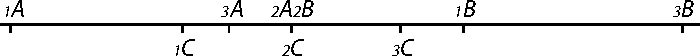
\includegraphics[width=0.79\textwidth]{gesamttex/edit_VIII,3/images/LH_35_09_21_001-002_d2.pdf}}%
  \vspace{0.5em}
  \centerline{\lbrack\textit{Fig.~2}\rbrack}%
  \label{LH_35_09_21_002r_Fig.2}%
%
\newpage
%
\pstart%
\textit{{\scriptsize1}A{\scriptsize2}A}, 5\textit{v}.\;
\textit{{\scriptsize1}B{\scriptsize2}B}, 4\textit{y}.\;
\textit{AC}, 3\textit{b}.\;
\textit{BC}, 6\textit{a}.\;
\textit{{\scriptsize1}C{\scriptsize2}C}, 2\textit{c}.\;
%
%\edtext{}{%
%\lemma{\textit{{\scriptsize2}A{\scriptsize3}A}, $-1\!\cdot\!x$}\Cfootnote{%
%Bei den folgenden Herleitungen gilt zuweilen aber \textit{{\scriptsize2}A{\scriptsize3}A} = $1 \!\cdot\! x$.
%Somit kommt \textit{{\scriptsize2}A{\scriptsize3}A} insgesamt der Wert $\pm\, 1 \!\cdot\! x$ zu.}}
\textit{{\scriptsize2}A{\scriptsize3}A}, $-1\!\cdot\!x.$\;
%
\textit{{\scriptsize2}B{\scriptsize3}B}, 8\textit{z}.
%
\edtext{}{%
\lemma{\textit{Am Rand:}}\Afootnote{%
$6 + 3 : 3 \squaredots 5 + 4 : 3,$
$6 + 3 : 6 \squaredots 5 + 4 : 6$%
\newline%
}}%
%
\pend%
%\newpage%
%
\pstart%
%
\edtext{}{%
\lemma{\textit{Am Rand:}}\Afootnote{%
Paradoxum:%
\protect\index{Sachverzeichnis}{paradoxum}
duo corpora possunt se%
\textsuperscript{[a]}
directo concursu mutuo sistere,%
\protect\index{Sachverzeichnis}{corpora mutuo sistentia post concursum}%
\protect\index{Sachverzeichnis}{concursus directus}
quae tamen virium sint inaequalium.%
\protect\index{Sachverzeichnis}{vires inaequales corporum concurrentium}%
\protect\index{Sachverzeichnis}{corpora virium inaequalium}
Imo nisi sint aeque \lbrack celeria\rbrack%
\textsuperscript{[b]}
et \lbrack aequalia,\rbrack%
\textsuperscript{[c]}%
\protect\index{Sachverzeichnis}{corpora concurrentia aequalia}%
\protect\index{Sachverzeichnis}{corpora concurrentia aeque celeria}
semper inaequalium sunt virium absolutarum,%
\protect\index{Sachverzeichnis}{vis absoluta corporum concurrentium}
etsi respectivas ipsas habeant aequales.%
\protect\index{Sachverzeichnis}{vis respectiva corporum concurrentium}
Ita si%
\textsuperscript{[d]}
corpus unum ut 2 habeat celeritatem ut 1,%
\protect\index{Sachverzeichnis}{celeritas corporum concurrentium}
et alterum ut 1 celeritatem ut 2,
sistent sese,%
\protect\index{Sachverzeichnis}{corpora mutuo sistentia post concursum}
sed tamen vires habent inaequales,%
\protect\index{Sachverzeichnis}{vires inaequales corporum concurrentium}
nam prioris vis est 2,
posterioris est 4.%
\newline\vspace{-0.5em}%
\newline%
{\footnotesize%
\textsuperscript{[a]}~se
\textit{(1)}~directe
\textit{(2)}~directo%
~\textit{L}
%
\quad%
\textsuperscript{[b]}~celeres%
~\textit{L~ändert Hrsg.}%
%
\quad%
\textsuperscript{[c]}~aequales%
~\textit{L~ändert Hrsg.}%
%
\quad%
\textsuperscript{[d]}~si
\textit{(1)}~\textbar~corpus \textit{erg.}~%
\textbar\ 2.1 et 1.2 se s
\textit{(2)}~corpus unum
\textit{(a)}~habeat
\textit{(b)}~ut 2 habeat
\lbrack...\rbrack\ sistent sese%
~\textit{L}\vspace{-4mm}}}}%
%
\textit{A} autem sit corpus,
quod post centrum gr.%
\protect\index{Sachverzeichnis}{centrum gravitatis}
insequitur.%
\protect\index{Sachverzeichnis}{corpus centrum gravitatis insequens}
\pend%
%
\pstart%
$5v \;\pleibdashv\, 4y \stackrel{(1)}{=} 3b + 6a,$
ubi $\pleibdashv$ significat $+$
si corpora sibi occurrant;%
\protect\index{Sachverzeichnis}{corpora occurrentia}
at idem significat $-$
si in easdem partes tendant.%
\protect\index{Sachverzeichnis}{corpora in easdem partes tendentia}
\pend%
%\newpage%
%
\pstart%
$2c \stackrel{(2)}{=} 5v - 3b
\stackrel{(3)}{=}$ (per 1 et 2) $6a \;\pleibvdash\, 4y.$%
\edlabel{LH_35_09_21_001-002_c002r6}
%
\pend%
%
\pstart%
$-1\!\cdot\!x \stackrel{(4)}{=} 2c - 3b \stackrel{(5)}{=} 5v - (2)3b$
%\pend%
%%
%\pstart%
et
$(2)3b \stackrel{(6)}{=} 5v - \!\cdot \overline{-1\!\cdot\!x}.$
\pend%
%
\pstart%
$8z \stackrel{(7)}{=} 2c + 6a
\stackrel{(8)}{=} \;\pleibvdash\, 4y + (2)6a$ (per 3)
$\stackrel{(9)}{=} 5v - 3b + 6a$ (per 2 et 7)
\pend%
%
\pstart%
et
$(2)6a \stackrel{(10)}{=} \;\pleibdashv\, 4y + 8z$ (per 7 et 8),
%\pend%
%%
%\pstart%
et (per 4,~7) erit
$8z - \!\cdot \overline{-1\cdot x}\stackrel{(11)}{=} 6a + 3b.$
\pend%
%
\pstart%
Ergo (per 1)
$8z - \!\cdot \overline{-1\!\cdot\!x} \;\stackrel{(12)}{=} 5v \;\pleibdashv\, 4y$
%
\edtext{seu $5v + \overline{-1\!\cdot\!x} \;\stackrel{((12))}{=} \;\pleibvdash\, 4y + 8z.$}{%
\lemma{seu}\Bfootnote{\hspace{-0,5mm}%
$5v + \overline{-1\!\cdot\!x} \ \stackrel{((12))}{=} \;\pleibvdash\, 4y + 8z.$
\textit{erg.~L}}}
\pend%
%
\pstart%
$\pleibdashv\, 4y \stackrel{(13)}{=} 3b + 6a - 5v$
\edlabel{LH_35_09_21_001-002_c002r1}%
per~1,
%
\edtext{}{%
{\xxref{LH_35_09_21_001-002_c002r1}{LH_35_09_21_001-002_c002r2}}%
{\lemma{per 1,}\Bfootnote{%
\textit{(1)}~et $16y^2 = 9b^2 + 36ab - 30bv$
\textit{(2)}~et $16y^2 \stackrel{(14)}{=} 9b^2 + (2)18ab - (2)15bv$%
~\textit{L}}}}%
%
\pend%
%\newpage%
%
\pstart%
\noindent%
%\hspace{1mm}\hspace{-1mm}% Trick
%
%
\edtext{}{%
{\xxref{LH_35_09_21_001-002_c002r9}{LH_35_09_21_001-002_c002r10}}%
{\lemma{\textit{Nebenrechnung:}}\Afootnote{%
\protect\raisebox{-3.65em}{$\displaystyle\frac{%
\protect\begin{tabular}[t]{rrr}%
25&16&150\\
6&3&48\\
$\overline{150\protect\vphantom{l^l}}$&$\overline{48\protect\vphantom{l^l}}$&$\overline{198\protect\vphantom{l^l}}$
\protect\end{tabular}%
}{%
\protect\begin{tabular}{rrr}%
\phantom{5}1&64&192\\
6&3&6\\
$\overline{6\protect\vphantom{l^l}}$&$\overline{192\protect\vphantom{l^l}}$&$\overline{198\protect\vphantom{l^l}}$
\protect\end{tabular}}$%
}%
\newline%
}}}%
%
%
\raisebox{4,06mm}{et}%
%\edlabel{LH_35_09_21_001-002_c002r11}%
%\edlabel{LH_35_09_21_001-002_c002r9}%
\hspace{2,0mm}%
%
\setlength{\tabcolsep}{1.0pt}%
\begin{tabular}{lllllll}%
$16y^2 \stackrel{(14)}{=} \hspace{2,4mm} $
&
$9b^2 \ \, +$
&
$(2)18ab \ \; -$
&
$(2)15bv \ \ + \ $%
\edlabel{LH_35_09_21_001-002_c002r2}
&
$36a^2 \ \ - \ $
&
$(2)30av \ \, + \, $
&
$25v^2$
\\
\phantom{1}5
&
9
&
\phantom{(2)\,1}3
&
\phantom{(2)\,1}3
&
\phantom{3}3
&
\phantom{(2)\,3}6
&
\phantom{2}3
\quad
probatio per abj. XI%
\protect\index{Sachverzeichnis}{probatio}%
\\
\phantom{1}7 & 0 & \phantom{(2)\,1}0 & \phantom{(2)\,1}6 & \phantom{3}0 & \phantom{(2)\,3}3 & \phantom{2}7 \quad probatio per abj. IX%
\protect\index{Sachverzeichnis}{probatio}%
\protect\index{Sachverzeichnis}{abjectio}%
\\%
\end{tabular}%
\edtext{}{\lemma{abj.\,}\Cfootnote{\textit{abjectio}, d.h. Prüfmethode (nach Vielfachen von 9 oder 11).}}
%
%\newline
\pend%
\vspace{0.5em}%
%
\pstart%
\noindent%
\[ \left \{%
%
%\hspace{-1,0mm}%
\edlabel{LH_35_09_21_001-002_c002r9}%
\setlength{\tabcolsep}{0.5pt}%
\begin{tabular}{l}%
\hspace{-0,8mm}%
$\phantom{1}48by^2\stackrel{(15)}{=}$%
\\%
\hspace{-0,8mm}%
\phantom{15}4%
\\%
\hspace{-0,8mm}%
$150av^2\stackrel{(16)}{=}$%
\\%
\end{tabular}
\right .%
\hspace{-1,5mm}%
%
\left \{%
\setlength{\tabcolsep}{1.8pt}
\begin{tabular}{llllll}%
\hspace{-1,4mm}%
$\phantom{1}\!\stackrel{\text{VI}}{27}\!b^3\: +$
&%
%\hspace{-1,9mm}%
$(2)\!\stackrel{...}{54}\!ab^2\: -$
&%
%\hspace{-1,9mm}%
$(2)\!\stackrel{....}{45}\!b^2v\ +$
&%
%\hspace{-1,9mm}%
$\!\stackrel{.....}{108}\!a^2b\ -$
&%
%\hspace{-1,9mm}%
$(2)\!\stackrel{..}{90}\!abv\ +$
&%
%\hspace{-1,9mm}%
$\!\stackrel{\text{VII}}{75}\!bv^2$
\\%
\hspace{-1,0mm}%
\phantom{15}5
&%
%\hspace{-1,9mm}%
\phantom{(2)\,5}9
&%
%\hspace{-1,9mm}%
\phantom{(2)\,4}9
&%
%\hspace{-1,9mm}%
\phantom{10}9
&%
%\hspace{-1,9mm}%
\phantom{(2)\,9}7
&%
%\hspace{-1,9mm}%
\phantom{7}9 \quad proba per XI%
\protect\index{Sachverzeichnis}{proba}%
\\%
\hspace{-0,8mm}%
$\stackrel{.}{150}\!av^2$& & & & &
\\%
\end{tabular}%
\hspace{1,0mm}%
\right \}\]%
%\rule[0pt]{10mm}{0pt}
\pend%
\vspace{0.40em}%
%
\pstart%
%\newline
%\rule[0mm]{1mm}{0mm}%
$\shortparallel$%
\hspace{122mm}%
$\shortparallel$
\pend%
\vspace{0.35em}%
%
\pstart%
\noindent%
\[%
\left%
\{%
%\hspace*{5mm}% 
\setlength{\tabcolsep}{0.5pt}%
\begin{tabular}{l}
\hspace{-0,8mm}%
$\phantom{19}6ax^2 \stackrel{(17)}{=} $%
\\
\hspace{-0,8mm}%
\phantom{19}6%
\\
\hspace{-0,8mm}%
$192bz^2\stackrel{(18)}{=}$%
\\%
\end{tabular}%
\right .%
\hspace{-1,5mm}%
\left \{%
\setlength{\tabcolsep}{1.8pt}%
\begin{tabular}{llllll}%
\hspace{-0,9mm}%
$\stackrel{.}{150}\!av^2 \:-$
&
$(4)\!\stackrel{..}{90}\!abv \ +$
&
$(4)\!\stackrel{...}{54}\!ab^2$%
& & &
\\
\hspace{-1,0mm}%
\phantom{15}7
&
\phantom{(4)\,9}3
&
\phantom{(4)\,5}7
\quad
per XI%\scriptsize{}
& & &
\\
\hspace{-2,0mm}%
$\phantom{1}\stackrel{\text{VII}}{75}\!bv^2 \:-$
&
$(2)\!\stackrel{....}{45}\!b^2v \ +$
&
$(2)\!\stackrel{..}{90}\!abv \ +$
&
\hspace{-6,0mm}%
$\stackrel{\text{VI}}{27}\!b^3 \:-$
&
$(2)\!\stackrel{...}{54}\!ab^2 \: +$
&
$\stackrel{.....}{108}\!a^2b$%
\\%
\end{tabular}%
\hspace{20,0mm}%
\right%
\}\]%
\edlabel{LH_35_09_21_001-002_c002r10}%
%\newline
\pend%
\vspace{-0.5em}%
%
\pstart%
\noindent%
Patet valorem 15 $+$ val. 16 $=$ val. 17 $+$ val. 18.%
\protect\index{Sachverzeichnis}{valor}%
%
%\edlabel{LH_35_09_21_001-002_c002r12}%
%
%
\edtext{}{%
\lemma{\textit{Am Rand:}}\Afootnote{%
Difficultas,%
\protect\index{Sachverzeichnis}{difficultas}
quod videtur corpus eo magis reflecti%
\protect\index{Sachverzeichnis}{corpus reflexum post concursum}%
\protect\index{Sachverzeichnis}{reflexio corporis post concursum}
quo motum est celerius.%
\newline%
}}%
%
\pend%
\vspace{0.25em}%
%\newpage%
%
\pstart%
Habemus ergo
$150av^2 +\, 48by^2 \stackrel{(19)}{=} 6ax^2 +\, 192bz^2$
seu
$6a \,\cdot\, \overline{25v^2 - 1\!\cdot\!x^2}
\stackrel{(20)}{=}
3b \,\cdot\, \overline{64z^2 - 16y^2},$
quam dividendo per aeq. ((12)) fiet%
\protect\index{Sachverzeichnis}{aequatio}
%
%
\edtext{}{%
{\xxref{LH_35_09_21_001-002_c002r7}{LH_35_09_21_001-002_c002r8}}%
{\lemma{$3b \cdot \overline{\leibdashv\, 4y + 8z}.$}\Bfootnote{%
\textit{(1)}~Seu $6a \cdot 5v \;\pleibvdash\, 3b4y \stackrel{(22)}{=} 6a \cdot \overline{-1\!\cdot\!x} + 3b8z.$
\textit{(a)}~Se
\textit{(b)}~Quod
\textit{(c)}~Quae aequatio 22 significat
\textit{(aa)}~differentiam
\textit{(bb)}~differentias
\textit{(cc)}~summ\textlangle am\textrangle\
\textit{(dd)}~differentiam motuum contrariam vel
\textit{(aaa)}~summa\textlangle r\textrangle\
\textit{(bbb)}~quantitatum
\textit{(aaaa)}~motus
\textit{(bbbb)}~motuum contrariorum, vel
\textit{(aaaaa)}~summam
\textit{(bbbbb)}~differentiam
\textit{(ccccc)}~summam conspirantium esse eandem, ante aut post concursum,
\textit{(aaaaa-a) }seu ex
\textit{(bbbbb-b)}~patet autem ex 21
\textit{(2)}~Quod significat \lbrack...\rbrack\ post concursum.%
~\textit{L}}}}%
%
$6a \cdot \overline{5v - \overline{-1\!\cdot\!x}} \,\stackrel{(21)}{=}
\edlabel{LH_35_09_21_001-002_c002r7}%
3b \,\cdot \,\overline{\leibdashv\, 4y + 8z}.$
%
Quod significat
%
\edtext{%
corpora esse reciproce%
\protect\index{Sachverzeichnis}{corpora concurrentia}
ut summas vel differentias suarum velocitatum%
\protect\index{Sachverzeichnis}{summa velocitatum corporum concurrentium}%
\protect\index{Sachverzeichnis}{differentia velocitatum corporum concurrentium}
ante et post concursum.%
\protect\index{Sachverzeichnis}{concursus corporum}%
\edlabel{LH_35_09_21_001-002_c002r8}
}{%
\lemma{\textit{Am Rand:}}\Afootnote{%
$6a : 3b \: \squaredots \; \pleibdashv\, 4y + 8z : 5v - \overline{-1\!\cdot\!x} \: \squaredots \: 3b + 6a - 5v + 5v - 3b + 6a : +\, 5v - 5v + (2)3b.$\vspace{-5mm}%
%\newline%
}}
%
%\edtext{}{%
%{\xxref{LH_35_09_21_002r_gstrmarg-1}{LH_35_09_21_002r_gstrmarg-2}}%
%{\lemma{\textit{Am Rand, gestrichen:}}\Afootnote{%
%{\footnotesize%
%Si sumas ${\scriptstyle \textit{1}}AE={\scriptstyle \textit{1}}C{\scriptstyle \textit{2}}C$}
%\lbrack\textit{Text bricht ab.}\rbrack}}}
%
\edtext{%
\edlabel{LH_35_09_21_002r_gstrmarg-1}%
Seu in
\edtext{figura praesenti%
\protect\index{Sachverzeichnis}{figura}%
}{%
\lemma{figura praesenti}\Cfootnote{%
Das Diagramm \lbrack\textit{Fig.~2}\rbrack\ auf S.~\pageref{LH_35_09_21_002r_Fig.2}.}}
$3b:6a\squaredots {\scriptstyle\textit{1}}A {\scriptstyle\textit{2}}A +{\scriptstyle\textit{2}}A {\scriptstyle\textit{3}}A : {\scriptstyle\textit{1}}B {\scriptstyle\textit{2}}B + {\scriptstyle\textit{2}}B {\scriptstyle\textit{3}}B.$%
\edlabel{LH_35_09_21_002r_gstrmarg-2}
\newline%
\indent%
Sed ut sciamus
quando summae aut differentiae
sunt adhibendae%
\lbrack,\rbrack%
}{%
\lemma{Seu}\Bfootnote{%
\textit{(1)}~$AC : BC \; \squaredots \ 6a : 3$
\textit{(2)}~in figura % praesenti $3b : 6a$ ...
\lbrack...\rbrack\ ${\scriptstyle\textit{1}}B {\scriptstyle\textit{2}}B + {\scriptstyle\textit{2}}B {\scriptstyle\textit{3}}B.$
\textit{(a)}~. Hinc
\textit{(b)}~sed ut \lbrack...\rbrack\ sunt adhibendae%
~\textit{L}}}
%
generale prodit pronuntiatum memorabile et paradoxum%
\protect\index{Sachverzeichnis}{pronuntiatum memorabile}%
\protect\index{Sachverzeichnis}{pronuntiatum paradoxum}%
\lbrack:\rbrack\
Si corpus post ictum%
\protect\index{Sachverzeichnis}{ictus}
regrediatur,%
\protect\index{Sachverzeichnis}{corpus regrediens post ictum}%
\protect\index{Sachverzeichnis}{regressus corporis post ictum}
summae,%
\protect\index{Sachverzeichnis}{summa velocitatum corporum concurrentium}
si progrediatur,%
\protect\index{Sachverzeichnis}{corpus progrediens post ictum}%
\protect\index{Sachverzeichnis}{progressus corporis post ictum}
differentiae velocitatum%
\protect\index{Sachverzeichnis}{differentia velocitatum corporum concurrentium}
(\protect\vphantom)%
seu spatiorum aequali tempore ante et post ictum percursorum%
\protect\index{Sachverzeichnis}{spatium percursum ante ictum}%
\protect\index{Sachverzeichnis}{spatium percursum post ictum}%
\protect\vphantom()
sunt corporibus reciproce proportionales.
Quod paradoxum,%
\protect\index{Sachverzeichnis}{paradoxum}
cum contrarium fieri debere videatur.
Sed res in ordinem rectum%
\protect\index{Sachverzeichnis}{ordo rectus}
%
\edtext{restituitur si}{%
\lemma{restituitur}\Bfootnote{%
\textit{(1)}~in aequ. \textlangle\textendash\textrangle\
\textit{(2)}~si%
~\textit{L}}}
%
\lbrack2~v\textsuperscript{o}\rbrack\ % % % %    Blatt 2v
%
non conjungamus in unum ejusdem
%
\edtext{corporis velocitates%
\protect\index{Sachverzeichnis}{velocitas ante ictum}%
\protect\index{Sachverzeichnis}{velocitas post ictum}
vel motus quantitates,%
\protect\index{Sachverzeichnis}{quantitas motus ante ictum}%
\protect\index{Sachverzeichnis}{quantitas motus post ictum}
ante et post ictum;%
\protect\index{Sachverzeichnis}{ictus}
sed potius}{%
\lemma{corporis}\Bfootnote{%
\textit{(1)}~velocitates ante et post ictum; sed potius
\textit{(2)}~velocitates vel % motus quantitates, ante et post ictum; 
\lbrack...\rbrack\ sed potius%
~\textit{L}}}
%
amborum corporum motus quantitates
ante ictum;
et similiter amborum post ictum,%
\protect\index{Sachverzeichnis}{quantitas motus ante ictum}%
\protect\index{Sachverzeichnis}{quantitas motus post ictum}
et fiet aequatio%
\protect\index{Sachverzeichnis}{aequatio}
talis:
\newline%
\centerline{%
$6a5v \;\pleibvdash\, 3b4y \stackrel{(22)}{=} 6a \cdot \overline{-1\!\cdot\!x} + 3b8z.$}
\newline%
Quod
%
\edtext{significat quantitatem progressus%
\protect\index{Sachverzeichnis}{quantitas progressus}
esse eandem ante et post ictum.%
\protect\index{Sachverzeichnis}{ictus}
Quantitatem autem progressus%
\protect\index{Sachverzeichnis}{quantitas progressus}
voco summam quantitatum motus,%
\protect\index{Sachverzeichnis}{summa quantitatum motus}
si duo corpora directione conspirant,%
\protect\index{Sachverzeichnis}{corpora directione conspirantia}
differentiam,%
\protect\index{Sachverzeichnis}{differentia quantitatum motus}
si directiones contrarias
%\edlabel{LH_35_09_21_001-002_c002v1}%
habent.%
\protect\index{Sachverzeichnis}{corpora directionem contrariam habentia}%
}{%
\lemma{significat}\Bfootnote{%
\textit{(1)}~summam quantitatum motus conspirantium, vel differen
\textit{(2)}~quantitatem progressus % esse eandem ante et post ictum. Quantitatem autem progressus voco summam quantitatum motus, si 
\lbrack...\rbrack\ duo corpora
\textit{(a)}~motu conspirant
\textit{(b)}~directione conspirant, % differentiam si directiones 
\lbrack...\rbrack\ contrarias habent.%
~\textit{L}}}
%
\pend%
\vspace{0.8em}%
%\newpage%
%
\pstart%
\noindent%
\lbrack\textit{Nachfolgend kleingedruckter Text in L gestrichen:}\rbrack\
\pend%
\vspace{0.5em}%
%
\footnotesize%
\pstart%
%
%\edtext{}{%
%{\xxref{LH_35_09_21_001-002_c002v1}{LH_35_09_21_001-002_c002v2}}%
%{\lemma{habent.}\Bfootnote{%
%\textit{(1)}~
Differentia%
\protect\index{Sachverzeichnis}{differentia velocitatum corporum concurrentium}
%
\edtext{velocitatum ejusdem corporis ante}{%
\lemma{velocitatum}\Bfootnote{%
\textit{(1)}~ante
\textit{(2)}~ejusdem corporis ante%
~\textit{L}}}
%
ictum et post ictum
est dupla velocitas centri%
\protect\index{Sachverzeichnis}{velocitas centri gravitatis}
%
\edtext{gravitatis%
\lbrack,\rbrack\
nam diff. inter 5\textit{v} et 1\textit{}x $\stackrel{(23)}{\text{est}}$ (2)2\textit{c},
nam $5v-1x=$}{%
\lemma{gravitatis}\Bfootnote{%
\textit{(1)}~\textlangle et\textrangle\
\textit{(2)}~nam
\textit{(a)}~\textit{dy} et \textit{z}
\textit{(b)}~diff. inter
\textit{(aa)}~5v et \textit{x}
\textit{(bb)}~5\textit{v}
\textit{(aaa)}~et $-\, \langle\overline{1-x}\rangle$
\textit{(bbb)}~et 1\textit{x} $\stackrel{(23)}{\text{est}}$
\textit{(aaaa)}~4 $+$
\textit{(bbbb)}~(2)2\textit{c},
\textit{(aaaaa)}~et diff. inter $4y$ et
\textit{(bbbbb)}~nam $5v - 1x=$%
~\textit{L}}}
%
{\normalsize%
\lbrack\textit{Text bricht ab.}\rbrack%
}%
\pend%
\vspace{0.5em}
%
\normalsize%
\pstart%
Ex aeq. 2 et 4 fit:
$(2)2c \stackrel{(23)}{=} 5v + \overline{-1\!\cdot\!x},$
et ex aeq. 3 et 7 fit
$(2)2c = \;\pleibvdash\, 4y + 8z.$%
\protect\index{Sachverzeichnis}{aequatio}
%\edlabel{LH_35_09_21_001-002_c002v2}
Unde
%
\edtext{sequitur progrediendi velocitatem
(\protect\vphantom)%
quae est summa
%
velocitatum ante et post ictum%
\protect\index{Sachverzeichnis}{summa velocitatum ante ictum}%
\protect\index{Sachverzeichnis}{summa velocitatum post ictum}%
\protect\index{Sachverzeichnis}{ictus}
si sunt conspirantes,%
\protect\index{Sachverzeichnis}{velocitates conspirantes ante ictum}
differentia si sunt contrariae%
\protect\index{Sachverzeichnis}{velocitates contrariae ante ictum}%
\protect\vphantom()
esse aequalem duplae velocitati centri
%
gravitatis,%
\protect\index{Sachverzeichnis}{velocitas centri gravitatis}%
\protect\index{Sachverzeichnis}{centrum gravitatis}
adeoque in ambobus corporibus esse eandem,
seu quod eodem redit,
intervallum
\textit{{\scriptsize1}A{\scriptsize3}A} vel \textit{{\scriptsize1}B{\scriptsize3}B}
inter loca%
}{%
\lemma{sequitur}\Bfootnote{%
\textit{(1)}~velocitatem progrediendi in momento ictus esse aequalem duplae velocitati centri gravitatis, adeoque in utroque corpore eandem. Est summam
\textit{(2)}~progrediendi velocitatem % (\protect\vphantom) quae est summa velocitatum ante et post ictum si sunt conspirantes, differentia si sunt contrariae \protect\vphantom() esse aequalem duplae velocitati 
\lbrack...\rbrack\ centri gravitatis,
\textit{(a)}~seu
\textit{(aa)}~esse
\textit{(bb)}~quod eodem redit,
\textit{(b)}~adeoque in % ambobus corporibus esse eandem, seu quod eodem 
\lbrack...\rbrack\ redit intervallum
\textit{(aa)}~inter locum
\textit{(bb)}~\textit{{\scriptsize1}A{\scriptsize3}A} vel \textit{{\scriptsize1}B{\scriptsize3}B} inter
\textit{(aaa)}~locum
\textit{(bbb)}~loca%
~\textit{L}}}
%
ante ictum et post ictum%
\protect\index{Sachverzeichnis}{ictus}%
\protect\index{Sachverzeichnis}{intervallum locorum ante ictum}%
\protect\index{Sachverzeichnis}{intervallum locorum post ictum}
eodem temporis intervallo%
\protect\index{Sachverzeichnis}{intervallum temporis ante ictum}%
\protect\index{Sachverzeichnis}{intervallum temporis post ictum}
ab ictu
%
\edtext{remota,
seu progressum corporis toto tempore%
\protect\index{Sachverzeichnis}{progressus ante ictum}%
\protect\index{Sachverzeichnis}{progressus post ictum}
cujus medio factus est ictus%
\protect\index{Sachverzeichnis}{ictus}
esse aequalem progressui}{%
\lemma{remota}\Bfootnote{%
\textit{(1)}~esse aequale intervallo progres
\textit{(2)}~,~seu
\textit{(a)}~integrum
\textit{(b)}~progressum corporis \lbrack...\rbrack\ aequalem progressui%
~\textit{L}}}
%
centri gravitatis%
\protect\index{Sachverzeichnis}{progressus centri gravitatis ante ictum}%
\protect\index{Sachverzeichnis}{progressus centri gravitatis post ictum}
eodem tempore facto,%
\protect\index{Sachverzeichnis}{tempus in cujus medio est ictus}
ac proinde in ambobus corporibus esse
%
\edlabel{LH_35_09_21_001-002_c002v3}%
aequalem.%
%
\edtext{}{%
{\xxref{LH_35_09_21_001-002_c002v3}{LH_35_09_21_001-002_c002v4}}%
{\lemma{aequalem.}\Bfootnote{%
\textit{(1)}~Ut summa corporum ad unum corpus, ita summa
\textit{(2)}~Quantum corpus
\textit{(a)}~habet velocitatis totalis super propriam tantum ipsi
\textit{(b)}~tota velocitate % ante ictum excedit 
\lbrack...\rbrack\ velocitatem propriam
\textit{(aa)}~ante i
\textit{(bb)}~tantum idem%
~\textit{L}}}}
%
\pend%
%
\pstart%
Quantum corpus%
\protect\index{Sachverzeichnis}{corpora concurrentia}
tota velocitate ante ictum%
\protect\index{Sachverzeichnis}{velocitas ante ictum}
excedit velocitatem propriam%
\protect\index{Sachverzeichnis}{velocitas propria corporum concurrentium}%
\lbrack,\rbrack\
tantum idem%
\edlabel{LH_35_09_21_001-002_c002v4}
%
corpus tota velocitate post ictum%
\protect\index{Sachverzeichnis}{velocitas post ictum}
deficit infra velocitatem propriam.%
\protect\index{Sachverzeichnis}{velocitas propria corporum concurrentium}
Et contra;
quanta autem est
differentia velocitatis totalis%
\protect\index{Sachverzeichnis}{differentia velocitatis totalis a propria}%
\protect\index{Sachverzeichnis}{velocitas totalis  corporum concurrentium}
a propria in uno,%
\protect\index{Sachverzeichnis}{velocitas propria corporum concurrentium}
tanta est et in altero,
tam ante ictum,
quam post ictum.%
\protect\index{Sachverzeichnis}{ictus}
\pend%
%
\pstart%
Vis ictus\protect\index{Sachverzeichnis}{vis ictus} semper
%
\edtext{est $6a9bb+3b36aa,$}{%
\lemma{est}\Bfootnote{%
\textit{(1)}~$6a3b \; +$
\textit{(2)}~$a + b$
\textit{(3)}~2\textit{a}b
\textit{(4)}~$2\, \overline{a+ b}$
\textit{(5)}~2
\textit{(6)}~5a
\textit{(7)}~$6a9bb + 3b36aa,$%
~\textit{L}}}
%
seu
$\overline{6a + 3b}$ in $6a3b.$
\pend%
%
%\pstart%
%\edtext{%
%Differentia quantitatum motus totalium % ,
%est differentia quantitatum motus%
%\protect\index{Sachverzeichnis}{quantitas motus totalis}%
%\protect\index{Sachverzeichnis}{differentia quantitatum motus}
%centro gravitatis contraeuntium.%
%\protect\index{Sachverzeichnis}{centrum gravitatis}%
%\protect\index{Sachverzeichnis}{quantitas motus contraiens centro gravitatis}%
%}{%
%\lemma{Differentia}\Bfootnote{%
%\hspace{-0,5mm}quantitatum
%\lbrack...\rbrack\ gravitatis contraeuntium.
%\textit{erg.~L}}}
%\pend%
%\newpage
%\vspace{0.5em}%
%
\pstart%
\edtext{Differentia quantitatum motus%
\protect\index{Sachverzeichnis}{differentia quantitatum motus}}{%
\lemma{Differentia}\Bfootnote{%
\hspace{-0,5mm}quantitatum motus
\textit{erg.~L}}}%
\lbrack:\rbrack\
$6a5v + 3b4y - 6a1x - 3b8z,$
%
%\edtext{$6a5v - 3b4y - 6a1x - 3b8z,$%
%}{\lemma{$6a5v - 3b4y - 6a1x - 3b8z$}\Cfootnote{%
%Es wäre
%$6a5v \mp 3b4y + 6a1x - 3b8z$
%zu erwarten,
%wo $+\, 6a1x$ als $\pm 6a1x$ gilt.}}
%
ponendo
%
\edtext{pro \textit{x} rem ejus,}{%
\lemma{pro \textit{x}}\Bfootnote{%
\textit{(1)}~quantitatem
\textit{(2)}~unif
\textit{(3)}~molem
\textit{(4)}~rem ejus%
~\textit{L}}}
%
seu id affirmativum quod includit.
\pend%
%\newpage%
%
\pstart%
\edtext{}{%
{\xxref{LH_35_09_21_002v_lisays-1}{LH_35_09_21_002v_lisays-2}}%
{\lemma{Si}\Bfootnote{%
\hspace{-0,5mm}ambo
\lbrack...\rbrack\ ad oppositas
\textit{erg.~L}}}}%
Si%
\edlabel{LH_35_09_21_002v_lisays-1}
ambo corpora ante concursum et post concursum%
\protect\index{Sachverzeichnis}{concursus corporum}
tendant in easdem partes,%
\protect\index{Sachverzeichnis}{corpora in easdem partes tendentia}
quantitas motus%
\protect\index{Sachverzeichnis}{quantitas motus corporum concurrentium}
utrobique aequalis;%
\protect\index{Sachverzeichnis}{quantitas motus utrobique aequalis}
si ante concursum tendant ad easdem partes,%
\protect\index{Sachverzeichnis}{corpora in easdem partes tendentia}
non post,
tunc quantitas motus ante concursum%
\protect\index{Sachverzeichnis}{quantitas motus ante concursum}
aequalis differentiae post concursum,%
\protect\index{Sachverzeichnis}{differentia quantitatum motus}
cujus discrimen a summa%
\protect\index{Sachverzeichnis}{summa quantitatum motus}
est
%
\edtext{dupla quantitas motus corporis}{%
\lemma{dupla}\Bfootnote{%
\textit{(1)}~corporis
\textit{(2)}~quantitas motus corporis%
~\textit{L}}}
%
\edtext{minoris.%
\protect\index{Sachverzeichnis}{quantitas motus corporis minoris}%
}{\lemma{minoris}\Cfootnote{%
Gemeint ist wohl \textit{majoris}. Vgl. S.~\refpassage{LH_35_09_21_002_izgf-1}{LH_35_09_21_002_izgf-2}.}}
Itaque hoc
%
\edtext{casu%
\protect\index{Sachverzeichnis}{casus}
quantitas motus tota ante concursum%
\protect\index{Sachverzeichnis}{quantitas motus ante concursum}%
\protect\index{Sachverzeichnis}{quantitas motus tota}
excedit eam post concursum%
\protect\index{Sachverzeichnis}{quantitas motus excedens}
dupla quantitate motus post concursum%
\protect\index{Sachverzeichnis}{quantitas motus post concursum}%
\protect\index{Sachverzeichnis}{quantitas motus dupla}
corporis minorem habentis.%
\protect\index{Sachverzeichnis}{quantitas motus minor}%
}{%
\lemma{casu}\Bfootnote{%
\textit{(1)}~prodita est dupla
\textit{(2)}~qua
\textit{(3)}~discri
\textit{(4)}~quantitas motus \lbrack...\rbrack\ quantitate motus
\textit{(a)}~corporis
\textit{(b)}~post concursum corporis minorem habentis.%
~\textit{L}}}
%
Si ante concursum
tendant in contrarias partes,%
\protect\index{Sachverzeichnis}{corpora in partes contrarias tendentia}
post concursum ad easdem,%
\protect\index{Sachverzeichnis}{corpora in easdem partes tendentia}
lucrum quantitatis motus%
\protect\index{Sachverzeichnis}{lucrum quantitatis motus}%
\protect\index{Sachverzeichnis}{quantitas motus lucrata}
est duplum minorem habentis ante concursum.%
\protect\index{Sachverzeichnis}{quantitas motus minor}
%\lbrack,\rbrack\
Si ante et post concursum\protect\index{Sachverzeichnis}{concursus corporum}
ad oppositas%
\edlabel{LH_35_09_21_002v_lisays-2}
\lbrack\textit{Text bricht ab.}\rbrack%
\pend%
%\newpage%
%
\pstart%
Hinc
%
\edtext{ex aeq. 22%
\protect\index{Sachverzeichnis}{aequatio}%
}{%
\lemma{ex}\Bfootnote{%
\hspace{-0,5mm}aeq. 22
\textit{erg.~L}}}
%
patet,
si corpora tendant in eandem partem%
\protect\index{Sachverzeichnis}{corpora in easdem partes tendentia}
ante et post ictum,%
\protect\index{Sachverzeichnis}{ictus}
quantitatem motus%
\protect\index{Sachverzeichnis}{quantitas motus ante ictum}%
\protect\index{Sachverzeichnis}{quantitas motus post ictum}
%
\edtext{ante et post}{%
\lemma{ante}\Bfootnote{\hspace{-0,5mm}%
\textbar~et \textit{erg.}~%
\textbar\ post%
~\textit{L}}}
%
ictum fore eandem,
nam $\;\pleibvdash\,$ significat $+,$
et \textit{x} erit quantitas affirmativa,%
\protect\index{Sachverzeichnis}{quantitas motus affirmativa}
nec proinde praefigi illi debebit numerus $-\,1.$
Sin corpora tendant in diversas partes%
\protect\index{Sachverzeichnis}{corpora in partes diversas tendentia}
ante et post
%
\edtext{ictum,%
\protect\index{Sachverzeichnis}{ictus}
neutrius}{%
\lemma{ictum,}\Bfootnote{%
\textit{(1)}~\textbar~si \textit{streicht Hrsg.}~%
\textbar\ modo
\textit{(2)}~neutrius%
~\textit{L}}}
%
differentia erit aequalis summae,%
\protect\index{Sachverzeichnis}{differentia quantitatum motus}%
\protect\index{Sachverzeichnis}{summa quantitatum motus}
ita ut
summa sumta in eo statu
quo in easdem partes tendunt,
differentia
quando in oppositas.
\pend%
%
\pstart%
Aeq. 21%
\protect\index{Sachverzeichnis}{aequatio}
est pro velocitatibus%
\protect\index{Sachverzeichnis}{velocitas tanquam linea}
%
\edtext{tanquam lineis,}{%
\lemma{tanquam}\Bfootnote{%
\hspace{-0,5mm}lineis
\textit{erg.~L}}}
%
22 pro quantitatibus motus%
\protect\index{Sachverzeichnis}{quantitas motus tanquam planum}
tanquam planis,
19 pro viribus tanquam solidis.%
\protect\index{Sachverzeichnis}{vis tanquam solidum}
\pend%
%
\count\Bfootins=900%
\count\Afootins=1200%
\count\Cfootins=900 
\pstart%
Si duo corpora elastro carentia concurrant,%
\protect\index{Sachverzeichnis}{elastrum restituens}%
\protect\index{Sachverzeichnis}{corpus elastro carens}
amissis propriis velocitatibus%
\protect\index{Sachverzeichnis}{velocitas propria}
recipient communem,%
\protect\index{Sachverzeichnis}{velocitas communis}
ibuntque cum centro gravitatis%
\protect\index{Sachverzeichnis}{centrum gravitatis}
et coincident \textit{{\scriptsize3}A},
\textit{{\scriptsize3}B},
\textit{{\scriptsize3}C},
quia post ictum simul
%
\edtext{ibunt.
Porro eadem vim ictus%
\protect\index{Sachverzeichnis}{vis ictus}
perdere manifestum est,
tantum enim virium amittitur%
\protect\index{Sachverzeichnis}{vis amissa}
quantum in mollium compressionem,%
\protect\index{Sachverzeichnis}{compressio mollium}%
\protect\index{Sachverzeichnis}{corpus molle}%
\protect\index{Sachverzeichnis}{corpus compressum}
ex qua se non ut elastra restituunt,%
\protect\index{Sachverzeichnis}{elastrum restituens}%
\protect\index{Sachverzeichnis}{restitutio elastri}
impensum est.}{%
\lemma{ibunt.}\Bfootnote{%
\textit{(1)}~Cumque
\textit{(2)}~Eadem perdent vim ictus. Unde patet vim ictus et vim mollium post i
\textit{(3)}~Porro eadem
\lbrack...\rbrack\ elastra restituunt,
\textit{(a)}~impendit
\textit{(b)}~impensum est.%
~\textit{L}}}
%
Eaque vis absorbetur a mollium partibus,%
\protect\index{Sachverzeichnis}{pars mollis}%
\protect\index{Sachverzeichnis}{vis absorpta a partibus mollibus}
unde sequitur differentiam inter
%
\edtext{vim totam%
\protect\index{Sachverzeichnis}{vis tota}%
}{%
\lemma{vim}\Bfootnote{%
\textit{(1)}~ante ictum\protect\index{Sachverzeichnis}{ictus}
\textit{(2)}~totam%
~\textit{L}}}
%
et vim ictus%
\protect\index{Sachverzeichnis}{ictus}%
\protect\index{Sachverzeichnis}{vis ictus}%
\protect\index{Sachverzeichnis}{differentia inter vim totam et vim ictus}
esse vim corporum%
\protect\index{Sachverzeichnis}{vis corporum concurrentium}
si solum haberent motum communem,%
\protect\index{Sachverzeichnis}{motus communis corporum concurrentium}
seu productum corporum in
%
\edtext{quadratum celeritatis centri gravitatis.%
\protect\index{Sachverzeichnis}{quadratum celeritatis}%
\protect\index{Sachverzeichnis}{celeritas centri gravitatis}%
\protect\index{Sachverzeichnis}{centrum gravitatis}%
\protect\index{Sachverzeichnis}{productum corporis in quadratum celeritatis}
In singulis corporibus vera res est non in viribus,%
\protect\index{Sachverzeichnis}{vis corporis singuli}
sed in velocitatibus%
\protect\index{Sachverzeichnis}{velocitas corporis singuli}%
\lbrack,\rbrack\
ut velocitas tota%
\protect\index{Sachverzeichnis}{velocitas tota corporum concurrentium}
componitur ex communi%
\protect\index{Sachverzeichnis}{velocitas communis corporum concurrentium}
et propria%
\protect\index{Sachverzeichnis}{velocitas propria corporum concurrentium}%
}{%
\lemma{quadratum}\Bfootnote{%
\textit{(1)}~centri gravitatis
\textit{(2)}~celeritatis centri gravitatis. 
\textit{(a)}~Itaque ex vi 
\textit{(b)}~Idque non tantum verum est in
\textit{(aa)}~totis
\textit{(bb)}~ambobus corporibus
\textbar~verum \textit{erg. u. gestr.}~%
\textbar~, sed et in
\textit{(c)}~In singulis
\textit{(aa)}~non tantum
\textit{(bb)}~corporibus vera % res est non in viribus, sed 
\lbrack...\rbrack\ in velocitatibus
\textit{(aaa)}~nam $5v=2c+3b,$ et alterum $3b$ motus ejus
\textit{(bbb)}~ut velocitas % tota componitur ex communi 
\lbrack...\rbrack\ et propria%
~\textit{L}}}
%
si ambo tendant in easdem partes.%
\protect\index{Sachverzeichnis}{corpora in easdem partes tendentia}
Sed si
%
\edtext{\lbrack tendant\rbrack}{%
\lemma{tendat}\Bfootnote{%
\textit{L~ändert Hrsg.}}}
%
in contrarias%
\protect\index{Sachverzeichnis}{corpora in partes contrarias tendentia}%
\lbrack,\rbrack\
in corpore tantum in easdem cum centro gravitatis%
\protect\index{Sachverzeichnis}{centrum gravitatis}
partes tendente verum est % ;
velocitatem totam%
\protect\index{Sachverzeichnis}{velocitas tota corporum concurrentium}
esse summam propriae et%
\protect\index{Sachverzeichnis}{velocitas propria corporum concurrentium}
%
\edtext{communis.%
\protect\index{Sachverzeichnis}{velocitas communis corporum concurrentium}
In altero
velocitas composita erit
propriae et communis differentia.%
}{%
\lemma{communis.}\Bfootnote{%
\textit{(1)}~Sin
\textit{(a)}~c
\textit{(b)}~minus
\textit{(2)}~In altero velocitas
\textit{(a)}~tota erit haec
\textit{(b)}~composita erit % propriae et 
\lbrack...\rbrack\ communis differentia.%
~\textit{L}}}
%
Interim mirum est
in summa ita omnia compensari.
Sed res
\edlabel{LH_35_09_21_002v_ejzt-1}%
ex navis%
\protect\index{Sachverzeichnis}{navis}
motu%
\protect\index{Sachverzeichnis}{motus navis}
patet%
\lbrack:\rbrack%
%
\edtext{}{%
{\xxref{LH_35_09_21_002v_ejzt-1}{LH_35_09_21_002v_ejzt-2}}%
{\lemma{ex}\Bfootnote{%
\textit{(1)}~natura
\textit{(2)}~navis motu patet
\textit{(a)}~, et \textlangle erit\textrangle\
\textit{(b)}~Si $av + by$% = +\,ax + bz 
~\textit{L}}}}
%
\pend%
%
\pstart%
Si
%
\edlabel{LH_35_09_21_002v_ejzt-2}%
$av + by = +\,ax + bz$
differentia quantitatum motus nulla.%
\protect\index{Sachverzeichnis}{quantitas motus nulla}
\pend%
%
\pstart%
Si%
\edlabel{LH_35_09_21_002_izgf-1}
$av + by =
%
\edtext{-\,ax + bz$
tunc
$ax + [bz] - av - by = 2ax.$
Et prior quantitas motus major.%
\protect\index{Sachverzeichnis}{quantitas motus major}%
\edlabel{LH_35_09_21_002_izgf-2}%
}{%
\lemma{$-\,ax + bz$}\Bfootnote{%
\textit{(1)}~tunc $av + by - ax - by = \langle ax\rangle$
\textit{(2)}~tunc $ax +\: \textbar~by \: \text{\textit{ändert Hrsg.}}~\textbar\ - av - by = 2ax.$
\textbar~Et prior quantitas motus major. \textit{erg.}~\textbar%
~\textit{L}}}
%
\pend%
%
\pstart%
Si
$av - by = +\,ax + bz$
tunc
$ax +
\edtext{[bz]}{%
\lemma{\textit{bx}}\Bfootnote{%
\textit{L~ändert Hrsg.}}}
- av - by =
\edtext{\lbrack-\,2by\rbrack.}{\lemma{2\textit{by}}\Bfootnote{\textit{L~ändert Hrsg.}}}$
%
\edtext{Et posterior major.%
\protect\index{Sachverzeichnis}{quantitas motus major}%
}{%
\lemma{Et}\Bfootnote{%
\hspace{-0,5mm}posterior major.
\textit{erg.~L}}}
%
\pend%
%
\pstart%
Si
$av - by = -\,ax + bz$
%
\edtext{tunc
$av - bz = by - ax.$}{%
\lemma{tunc}\Bfootnote{%
\textit{(1)}~diff. inter $av + by$ et $ax + bz = 2by + 2ax,$ nam $av + by -\,\overline{av - by} = 2by$
\textit{(2)}~$av - bz = by - ax.$%
~\textit{L}}}
%
\pend%
%\newpage%
%
\pstart%
\noindent%
Ergo
$av + by - ax - bz$
ponendo $=H,$
fiet
$2by - 2ax = H.$
%
%\edtext{ }{%
%\lemma{$2by-2ax=H$}\Bfootnote{%
%\textit{(1)}~Generaliter
%\textit{(2)}~Generaliter\%
%~\textit{L}}}
%
%\pend%
%%
%\pstart%
Generaliter
$av \;\pleibdashv\, by = (\pleibdashv\!)\, ax + bz.$
Ergo
%
$av - bz = %
\edtext{(\pleibdashv\!)\, ax \;\pleibvdash\, by.$
Jam
$((\pleibdashv\!))\,H = av + by - ax - bz.$%
}{%
\lemma{$(\pleibdashv\!)\, ax \;\pleibvdash\, by.$}\Bfootnote{%
\textit{(1)}~Jam $av + by$ diff. $ax + bz = H.$ Ergo $H = by$
\textit{(2)}~Jam
\textit{(a)}~$((\pleibdashv\!))\,H = ((\pleibdashv\!))\,av \;((\pleibdashv\!))\,by \;((\pleibvdash\!))\,ax \;((\pleibvdash\!))\,bz$ 
\textit{(b)}~$((\pleibvdash\!))\,H = av + by - ax - bz.$%
~\textit{L}}}
%
Ergo $((\pleibdashv\!))\,H = by \;\pleibvdash\, by - ax \;(\pleibdashv\!)\,ax.$
\pend%
\newpage
%
\pstart%
Ergo si corpora eodem tendunt ante et post concursum,%
\protect\index{Sachverzeichnis}{concursus corporum}%
\protect\index{Sachverzeichnis}{corpora eodem tendentia}
\textit{H} est
%
\edtext{\lbrack nulla\rbrack.}{%
\lemma{null}%
\Bfootnote{%
\textit{L~ändert Hrsg.}}}
%
Si tantum ante vel tantum post concursum%
\protect\index{Sachverzeichnis}{concursus corporum}
in contrarias partes tendunt,%
\protect\index{Sachverzeichnis}{corpora in contrarias partes tendentia}
\textit{H} est dupla quantitas
%
\edtext{\lbrack motus\rbrack}{%
\lemma{motus}\Bfootnote{%
\textit{erg. Hrsg.}}}
%
corporis%
\lbrack,\rbrack\
ex iis
quae in
%
\edtext{\lbrack contrarias\rbrack}{%
\lemma{contraria}\Bfootnote{%
\textit{L~ändert Hrsg.}}}
%
tendunt%
\lbrack,\rbrack\
minorem quantitatem motus habentis.%
\protect\index{Sachverzeichnis}{quantitas motus minor}
Si ambo in contrarias partes ante et post concursum tendunt,%
\protect\index{Sachverzeichnis}{corpora in contrarias partes tendentia}
\textit{H} est differentia quantitatum motus%
\protect\index{Sachverzeichnis}{differentia quantitatum motus}
minorum ante et post concursum.%
\protect\index{Sachverzeichnis}{quantitas motus minor}
Generaliter differentia
%
\edtext{totarum}{%
\lemma{totarum}\Bfootnote{%
\textit{erg.~L}}}
%
quantitatum
%
\edtext{motus ante et post concursum,%
\protect\index{Sachverzeichnis}{concursus corporum}
est differentia singularium quantitatum motus%
\protect\index{Sachverzeichnis}{differentia quantitatum motus}
directioni centri gravitatis contrariarum,%
\protect\index{Sachverzeichnis}{quantitas motus directioni centri gravitatis contraria}
ubi quae contrariae non sunt
habentur pro nullis.%
\protect\index{Sachverzeichnis}{quantitas motus nulla}%
}{%
\lemma{motus}\Bfootnote{%
\textit{(1)}~est
\textit{(2)}~ante et % post concursum, 
\lbrack...\rbrack\ est differentia
\textit{(a)}~quan
\textit{(b)}~inter
\textit{(c)}~singularium quantitatum motus
\textit{(aa)}~duorum corporum
\textit{(bb)}~directioni centri gravitatis contrariarum,
\textit{(aaa)}~quarum \lbrack\textit{!}\rbrack\ ante concursum, alteram post concursum centro gravitatis contrariam
\textit{(bbb)}~ubi quae % contrariae non sunt habentur 
\lbrack...\rbrack\ pro nullis.%
~\textit{L}}}
%
Nullum corpus contrarium centro gravitatis%
\protect\index{Sachverzeichnis}{corpus contrarium centro gravitatis}
est tam ante quam post concursum.%
\protect\index{Sachverzeichnis}{concursus corporum}
\pend%
%
\pstart%
\edtext{%
Differentia quantitatum motus totalium % ,
est differentia quantitatum motus%
\protect\index{Sachverzeichnis}{quantitas motus totalis}%
\protect\index{Sachverzeichnis}{differentia quantitatum motus}
centro gravitatis contraeuntium.%
\protect\index{Sachverzeichnis}{centrum gravitatis}%
\protect\index{Sachverzeichnis}{quantitas motus contraiens centro gravitatis}%
}{%
\lemma{Differentia}\Bfootnote{%
\hspace{-0,5mm}quantitatum
\lbrack...\rbrack\ gravitatis contraeuntium.
\textit{erg.~L}}}
\pend%
\count\Bfootins=1200%
\count\Afootins=1200%
\count\Cfootins=1200 
%
%
%
%
% % % %    Ende des Stücks auf Blatt 2v